\documentclass[table]{beamer}
%[]中可以使用draft、handout、screen、transparency、trancompress、compress等参数

%指定beamer的模式与主题
\mode<presentation>
{
  \usetheme{Madrid}
%\usetheme{Boadilla}
%\usecolortheme{default}
%\usecolortheme{orchid}
%\usecolortheme{whale}
%\usefonttheme{professionalfonts}
}

%\usetheme{Madrid}
%这里还可以选择别的主题:Bergen, Boadilla, Madrid, AnnArbor, CambridgeUS, Pittsburgh, Rochester, Warsaw, ...
%有导航栏的Antibes, JuanLesPins, Montpellier, ...
%有内容的Berkeley, PaloAlto, Goettingen, Marburg, Hannover, ...
%有最小导航栏的Berlin, Ilmenau, Dresden, Darmstadt, Frankfurt, Singapore, Szeged, ...
%有章和节表单的Copenhagen, Luebeck, Malmoe, Warsaw, ...

%\usecolortheme{default}
%设置内部颜色主题(这些主题一般改变block里的颜色);这个主题一般选择动物来命名
%这里还可以选择别的颜色主题,如默认的和有特别目的的颜色主题default,structure,sidebartab,全颜色主题albatross,beetle,crane,dove,fly,seagull,wolverine,beaver

%\usecolortheme{orchid}
%设置外部颜色主题(这些主题一般改变title里的颜色);这个主题一般选择植物来命名
%这里还可以选择别的颜色主题,如默认的和有特别目的的颜色主题lily,orchid,rose

%\usecolortheme{whale}
%设置字体主题;这个主题一般选择海洋动物来命名
%这里还可以选择别的颜色主题,如默认的和有特别目的的颜色主题whale,seahorse,dolphin

%\usefonttheme{professionalfonts}
%类似的还可以定义structurebold,structuresmallcapsserif,professionalfonts

% 控制 beamer 的风格,可以根据自己的爱好修改
%\usepackage{beamerthemesplit} %使用 split 风格
%\usepackage{beamerthemeshadow} %使用 shadow 风格
%\usepackage[width=2cm,dark,tab]{beamerthemesidebar}

%插入音标
%\usepackage{tipa}
%\AtBeginDocument{
  %\renewcommand\textipa{\fontencoding{T3}\selectfont}
%}
%\AtBeginDocument{
  %\renewcommand\textipa[2][r]{{\fontfamily{cm#1}\tipaencoding #2}}
%}
%\renewenvironment{IPA}[1][r]
 %{\fontfamily{cm#1}\tipaencoding}
 %{}

% 设定英文字体
%\usepackage{fontspec}
% Fix bugs for fontspec in TeXLive2015
\ifdefined\suppressfontnotfounderror
  \expandafter\let\csname xetex_suppressfontnotfounderror:D\endcsname
    \suppressfontnotfounderror
\else
  \expandafter\let\csname xetex_suppressfontnotfounderror:D\endcsname
    \luatexsuppressfontnotfounderror
\fi
\usepackage[no-math]{fontspec}
\setmainfont{Times New Roman}
\setsansfont{Arial}
\setmonofont{Courier New}

% 设定中文字体
\usepackage[BoldFont,SlantFont,CJKchecksingle,CJKnumber]{xeCJK}
%\setCJKmainfont[BoldFont={Adobe Heiti Std},ItalicFont={Adobe Kaiti Std}]{Adobe Song Std}
\setCJKmainfont[BoldFont={Adobe Heiti Std},ItalicFont={Adobe Kaiti Std}]{WenQuanYi Micro Hei}
\setCJKsansfont{Adobe Heiti Std}
\setCJKmonofont{Adobe Fangsong Std}
\punctstyle{hangmobanjiao}

\defaultfontfeatures{Mapping=tex-text}
\usepackage{xunicode}
\usepackage{xltxtra}

\XeTeXlinebreaklocale "zh"
\XeTeXlinebreakskip = 0pt plus 1pt minus 0.1pt

\usepackage{setspace}
\usepackage{colortbl,xcolor}
\usepackage{hyperref}
%\hypersetup{xetex,bookmarksnumbered=true,bookmarksopen=true,pdfborder=1,breaklinks,colorlinks,linkcolor=blue,filecolor=black,urlcolor=cyan,citecolor=green}
\hypersetup{xetex,bookmarksnumbered=true,bookmarksopen=true,pdfborder=1,breaklinks,colorlinks,linkcolor=cyan,filecolor=black,urlcolor=blue,citecolor=green}

% 插入图片
\usepackage{graphicx}
\graphicspath{{figures/}}
% 图文混排
%\usepackage{picins}
\usepackage{floatflt}

% 可能用到的包
\usepackage{amsmath,amssymb}
%插入多媒体
%\usepackage{media9}
%\usepackage{movie15}
\usepackage{multimedia}
\usepackage{multicol}
\usepackage{multirow}

% 定义一些自选的模板,包括背景、图标、导航条和页脚等,修改要慎重
% 设置背景渐变由10%的红变成10%的结构颜色
%\beamertemplateshadingbackground{red!10}{structure!10}
%\beamertemplatesolidbackgroundcolor{white!90!blue}
% 使所有隐藏的文本完全透明、动态,而且动态的范围很小
\beamertemplatetransparentcovereddynamic
% 使itemize环境中变成小球,这是一种视觉效果
\beamertemplateballitem
% 为所有已编号的部分设置一个章节目录,并且编号显示成小球
\beamertemplatenumberedballsectiontoc
% 将每一页的要素的要素名设成加粗字体
\beamertemplateboldpartpage

% item逐步显示时,使已经出现的item、正在显示的item、将要出现的item呈现不同颜色
\def\hilite<#1>{
 \temporal<#1>{\color{gray}}{\color{blue}}
    {\color{blue!25}}
}

\renewcommand{\today}{\number\year 年 \number\month 月 \number\day 日}

%五角星
\usepackage{MnSymbol}

%去除图表标题中的figure等
\usepackage{caption}
\captionsetup{labelformat=empty,labelsep=none}

\usepackage{tabu}
\usepackage{multirow}
%表格自动换行
\usepackage{tabularx} 

% 千分号
%\usepackage{textcomp}

%罗马数字
\makeatletter
\newcommand{\rmnum}[1]{\romannumeral #1}
\newcommand{\Rmnum}[1]{\expandafter\@slowromancap\romannumeral #1@}
\makeatother

%分栏
\usepackage{multicol}

%\usepackage{enumitem}
%\usepackage{enumerate}

%键盘
\usepackage{keystroke}

%心形
\usepackage{fdsymbol}

%插入源代码
\usepackage{listings}
\lstset{
  language=perl,                  % 程序语言名称:TeX, Perl, R, sh, bash, Awk
  basicstyle=\normalsize\tt,      %\tt指monospace字体族,程序源代码使用此族字体表示更加美观
  numbers=left,                   % 行号位置(左侧)
  numberstyle=\small,             % 行号字体的字号
  stepnumber=1,                   % 行号的显示步长
  numbersep=5pt,                  % 行号与代码间距
  backgroundcolor=\color{white},  % 背景色;需要 \usepackage{color}
  showspaces=false,               % 不显示空格
  showstringspaces=false,         % 不显示代码字符串中的空格标记
  showtabs=false,                 % 不显示 TAB
  tabsize=4, 
  frame=shadowbox,                % 把代码用带有阴影的框圈起来
  captionpos=b,                   % 标题位置
  breaklines=true,                % 对过长的代码自动断行
  breakatwhitespace=false,        % 断行只在空格处
  extendedchars=false,            % 解决代码跨页时,章节标题,页眉等汉字不显示的问题
  %escapeinside={\%*}{*},         % 跳脱字符,添加注释,暂时离开 listings 
  %escapeinside=``,
  commentstyle=\color{red!50!green!50!blue!50}\tt,  %浅灰色的注释
  rulesepcolor=\color{red!20!green!20!blue!20},     %代码块边框为淡青色
  keywordstyle=\color{blue!70}\bfseries\tt,         %代码关键字的颜色为蓝色,粗体
  identifierstyle=\tt,
  stringstyle=\tt,                % 代码字符串的特殊格式
  keepspaces=true,
  breakindent=1em,
  %breakindent=22pt,
  %breakindent=4em,
  breakautoindent=true,
  flexiblecolumns=true,
  aboveskip=1em,                  %代码块边框
  xleftmargin=2em,
  xrightmargin=2em
}

%\setbeamercolor{alerted text}{fg=magenta}
\setbeamercolor{bgcolor}{fg=yellow,bg=cyan}
%\setbeamercolor{itemize/enumerate body}{fg=green}

\begin{document}

%\includeonlyframes{current}

\logo{\includegraphics[height=0.08\textwidth]{tijmu.png}}

% 在每个Section前都会加入的Frame
\AtBeginSection[]
{
  \begin{frame}<beamer>
    %\frametitle{Outline}
    \frametitle{教学提纲}
    \setcounter{tocdepth}{3}
    \begin{multicols}{2}
      \tableofcontents[currentsection,currentsubsection]
      %\tableofcontents[currentsection]
    \end{multicols}
  \end{frame}
}
% 在每个Subsection前都会加入的Frame
\AtBeginSubsection[]
{
  \begin{frame}<beamer>
%%\begin{frame}<handout:0>
%% handout:0 表示只在手稿中出现
    \frametitle{教学提纲}
    \setcounter{tocdepth}{3}
    \begin{multicols}{2}
    \tableofcontents[currentsection,currentsubsection]
    \end{multicols}
%% 显示在目录中加亮的当前章节
  \end{frame}
}

% 为当前幻灯片设置背景
%{
%\usebackgroundtemplate{
%\vbox to \paperheight{\vfil\hbox to
%\paperwidth{\hfil\includegraphics[width=2in]{tijmu_charcoal.png}\hfil}\vfil}
%}
\begin{frame}[plain]
  \begin{center}
    {\Huge 分子生物计算\\}
    {\huge \textit{(Perl语言编程)}\\}
    \vspace{1cm}
    {\LARGE 天津医科大学\\}
    %\vspace{0.2cm}
    {\LARGE 生物医学工程与技术学院\\}
    \vspace{1cm}
    {\large 2019-2020学年上学期(秋)\\ 2017级生信班}
  \end{center}
\end{frame}
%}



\title[突变和随机化]{第七章\quad 突变和随机化}
\author[Yixf]{伊现富(Yi Xianfu)}
\institute[TIJMU]{天津医科大学(TIJMU)\\ 生物医学工程与技术学院}
\date{2019年10月}


\input{snippet/beamer_toc.tex}


\section{引言}
\begin{frame}
  \frametitle{突变和随机化 | 突变}
  \begin{block}{突变}
突变(mutation,即基因突变),指细胞中的遗传基因(通常指存在于细胞核中的脱氧核糖核酸)发生的改变。它包括单个碱基改变所引起的点突变,或多个碱基的缺失、重复和插入。
  \end{block}
  \pause
  \vspace{-0.5em}
  \begin{block}{原因}
    细胞分裂时遗传基因的复制发生错误、或受化学物质、毒性、辐射或病毒的影响等。
  \end{block}
  \pause
  \vspace{-0.5em}
  \begin{block}{影响}
    \begin{itemize}
      \item 突变通常会导致细胞运作不正常或死亡,甚至可以在较高等生物中引发癌症。
      \item 同时,突变也被视为物种进化的“推动力”:不理想的突变会经自然选择过程被淘汰,而对物种有利的突变则会被累积下去。中性突变(neutral mutation)对物种没有影响而逐渐累积,会导致间断平衡(punctuated equilibrium)。
    \end{itemize}
  \end{block}
\end{frame}

\begin{frame}
  \frametitle{突变和随机化 | 突变 | 类型}
  \begin{figure}
    \centering
    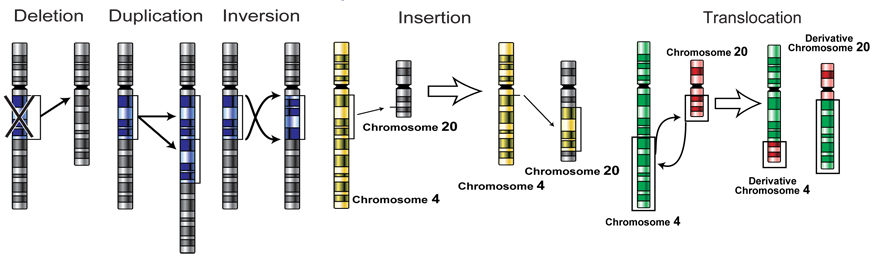
\includegraphics[width=\textwidth,height=0.6\textheight]{c7_mutation_type.png}
  \end{figure}
\end{frame}

\begin{frame}
  \frametitle{突变和随机化 | 突变 |点突变}
  \begin{figure}
    \centering
    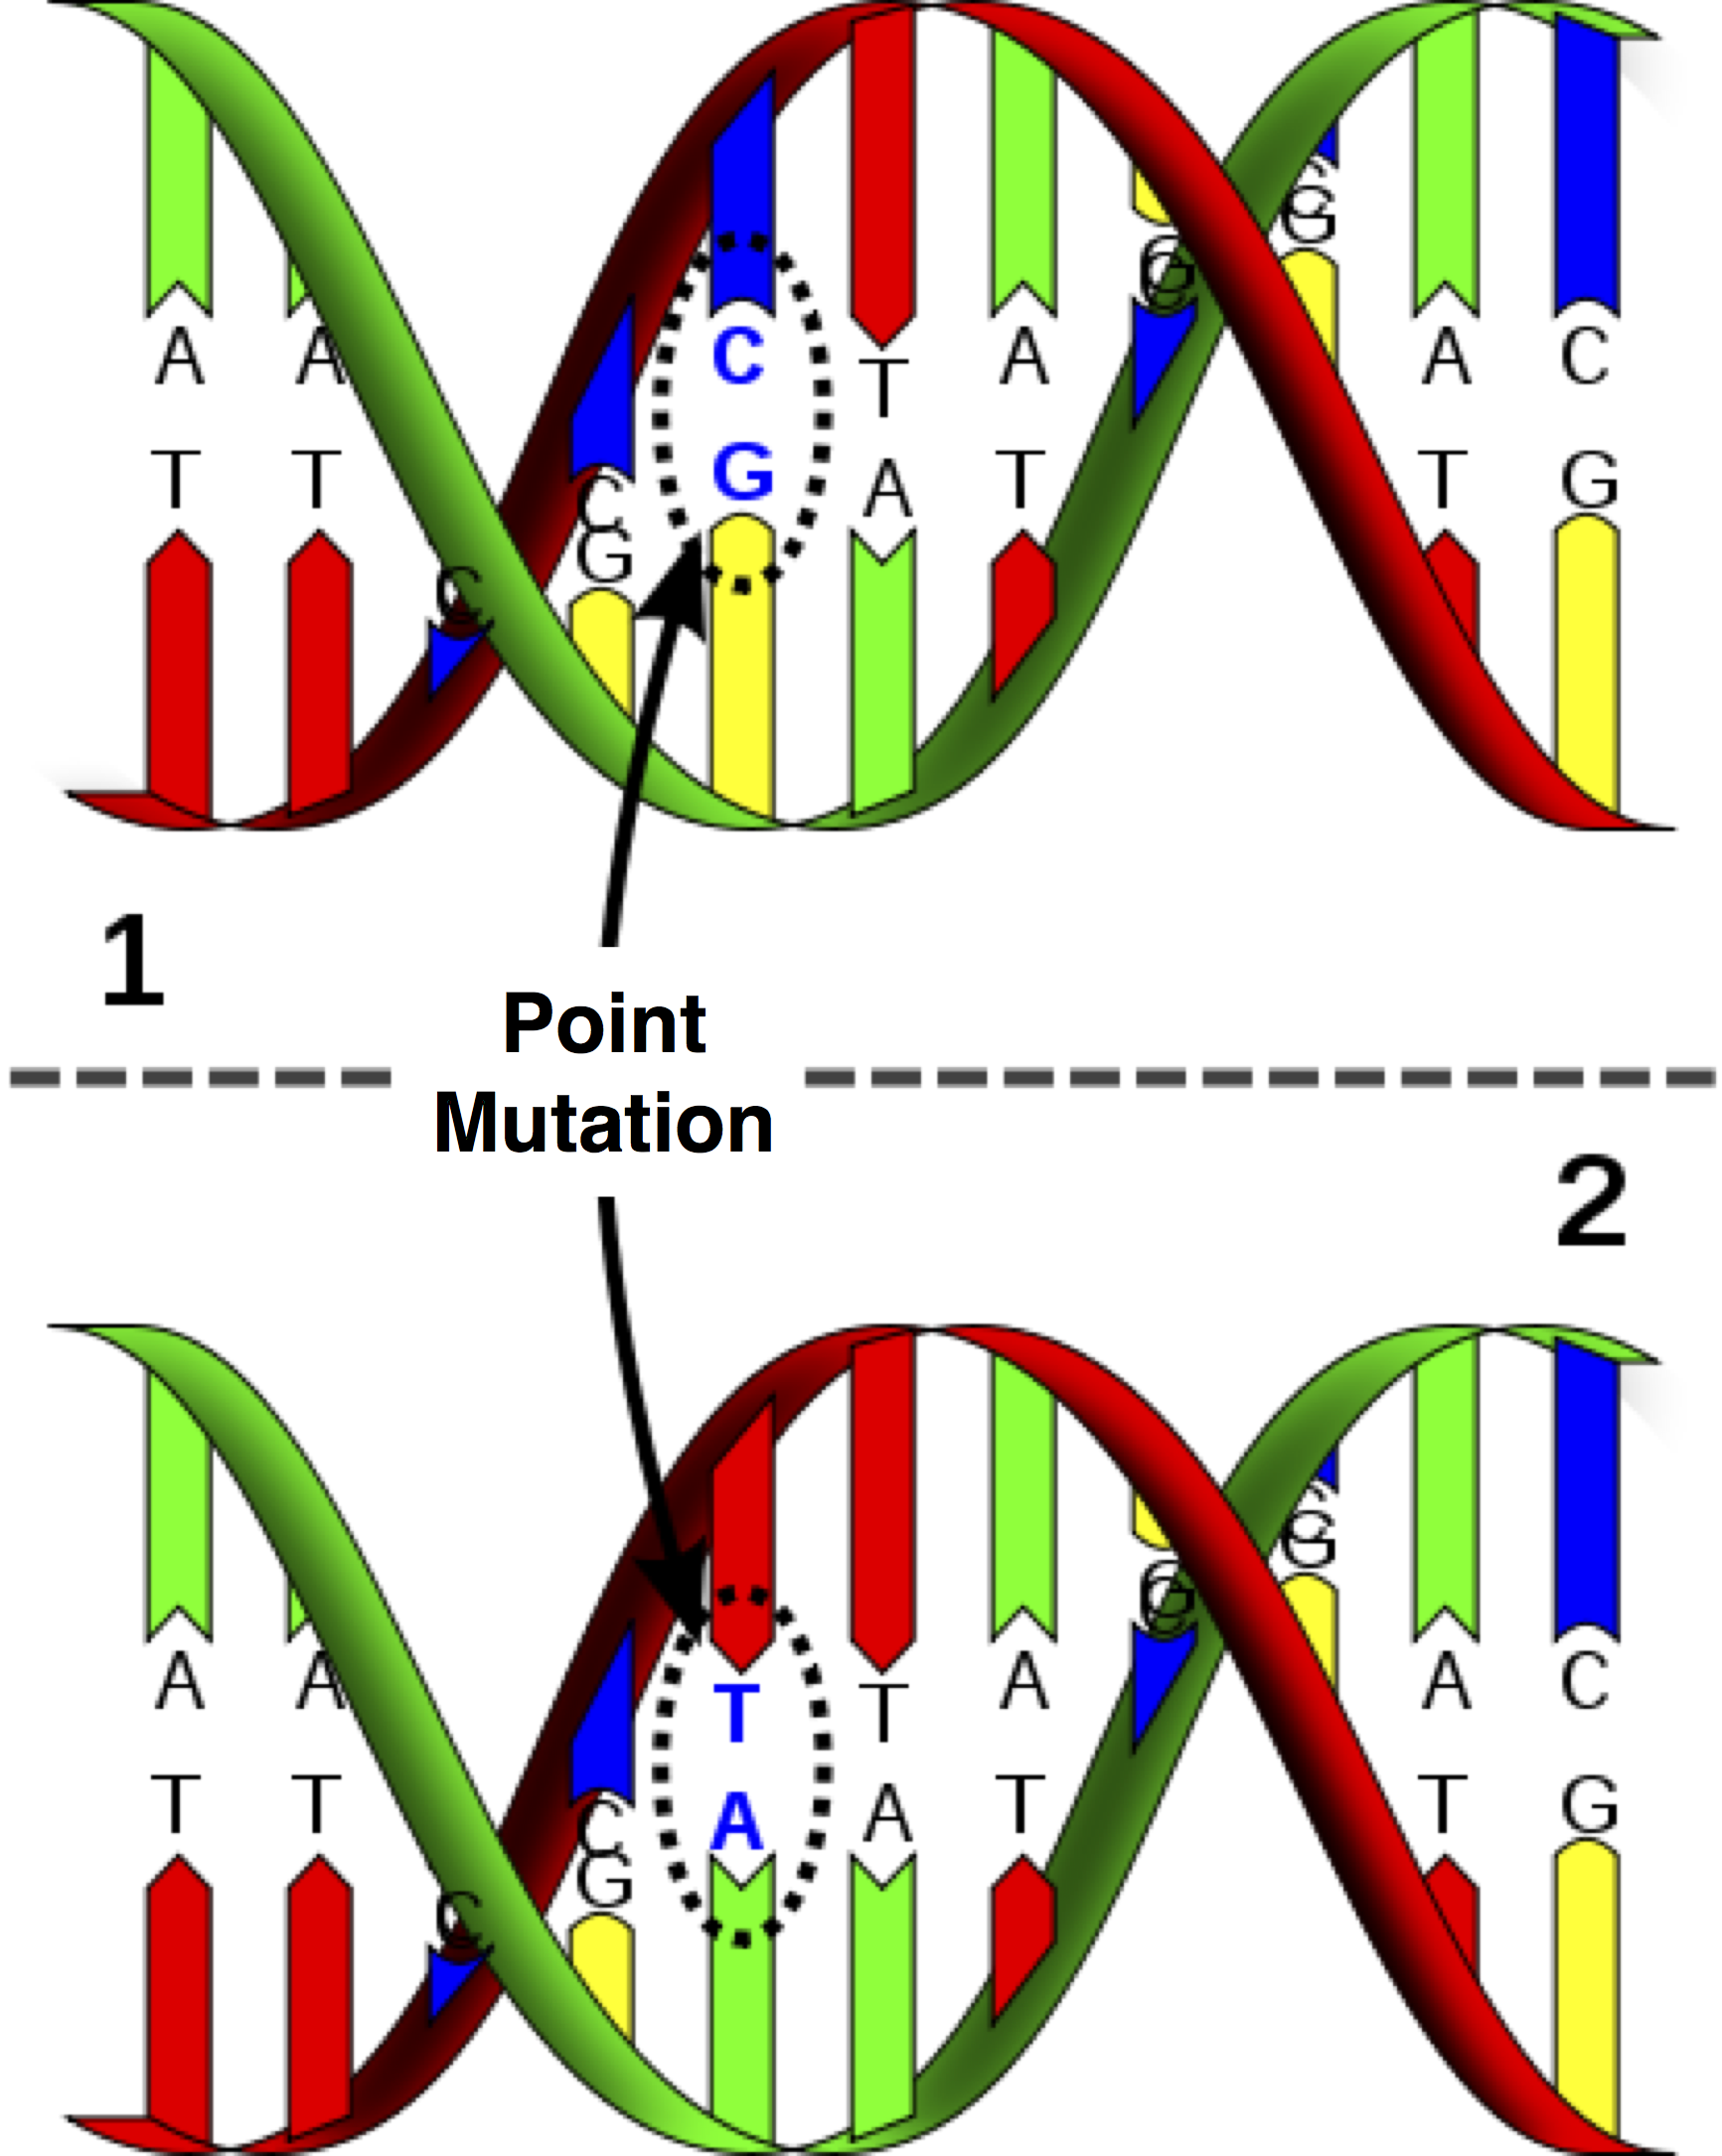
\includegraphics[width=0.8\textwidth,height=0.8\textheight]{c7_mutation_point_03.png}
  \end{figure}
\end{frame}

\begin{frame}
  \frametitle{突变和随机化 | 突变 | \alert{点突变}}
  \begin{block}{点突变}
 点突变(point mutation)是突变的一种类型,在遗传材料DNA或RNA中,会使单一碱基核苷酸替换成另一种核苷酸。通常这个术语也包括只作用于单一碱基对的插入或删除。 
  \end{block}
  \pause
  \begin{block}{分类}
    \begin{itemize}
      \item 转换/颠换:转换(Alpha)和颠换(Beta)在突变速率有系统的差异,转换突变大于颠换突变约10倍以上。
	\begin{itemize}
	  \item 转换:嘌呤替换另一个嘌呤,或嘧啶替换另一个嘧啶
	  \item 颠换:嘌呤替换嘧啶,嘧啶替换嘌呤
	\end{itemize}
      \item 功能
	\begin{itemize}
	  \item 无义突变(nonsense mutation):使原本可制造蛋白质的密码变成终止密码
	  \item 错义突变(missense mutation):使密码所对应的氨基酸改变
	  \item 无表型突变(silent mutation):密码改变,但对应的氨基酸不变
	\end{itemize}
    \end{itemize}
  \end{block}
\end{frame}

\begin{frame}
  \frametitle{突变和随机化 | 突变 | 点突变 | 类型}
  \begin{figure}
    \centering
    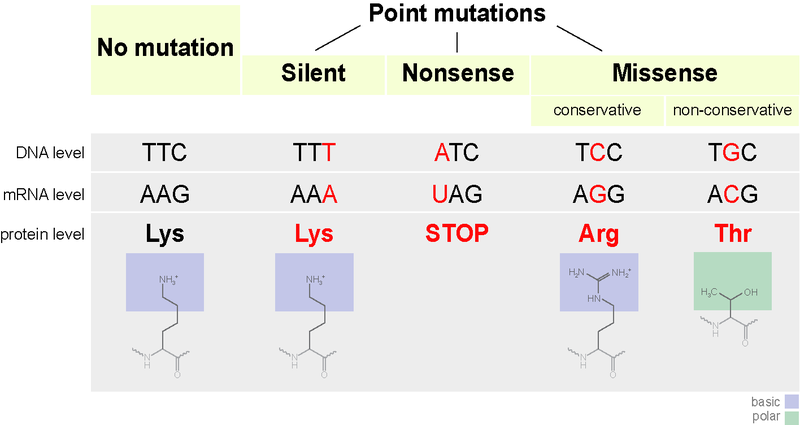
\includegraphics[width=0.9\textwidth]{c7_mutation_point_01.png}
  \end{figure}
\end{frame}

\begin{frame}
  \frametitle{突变和随机化 | 随机}
  \begin{block}{随机性}
    随机性(randomness)这个词是用来表达目的、动机、规则或一些非科学用法的可预测性的缺失。一个随机的过程是一个不定因子不断产生的重复过程,但它可能遵循某个概率分布。\\
    \vspace{1em}
随机经常用于统计学中,表示一些定义清晰的、彻底的统计学属性,例如缺失偏差或者相关。随机与任意不同,因为“一个变量是随机的”表示这个变量遵循概率分布。而任意在另一方面又暗示了变量没有遵循可限定概率分布。
  \end{block}
  \pause
  \begin{block}{科学与随机}
    在自然与工程学里一些现象会通过随机性模型来模拟:
    \begin{itemize}
      \item 混沌理论,密码学,博弈论,信息论,量子力学,模式识别
      \item 统计学,概率论,统计力学
    \end{itemize}
  \end{block}
\end{frame}

\begin{frame}
  \frametitle{突变和随机化 | 突变和随机}
  进化论将观察到的生命多样性归因于随机突变。由于一些突变的基因带给了拥有它们的个体更高的存活与繁衍的机会,随机突变保留在了基因库中。\\
  \vspace{1em}
生物体的特征在某种程度上是确定性地发生的(例如:在基因和环境的影响下),在某种程度上是随机发生的。例如,基因与曝光量仅仅支配着人体皮肤上出现的色斑密度;而单个色斑的精确位置看来是随机决定的。
\end{frame}

\begin{frame}
  \frametitle{突变和随机化 | 模拟}
  \begin{block}{模拟}
    模拟(simulation),泛指基于实验或训练为目的,将原本的事务或流程,予以系统化与公式化,以便进行可重现预期结果的模拟。
  \end{block}
  \pause
  \begin{block}{随机化模拟突变}
    \begin{itemize}
      \item 研究DNA突变的机制
      \item 研究突变对相关蛋白质生物活性的影响
      \item 有助于进化、疾病以及DNA分裂和修复机制等基本细胞过程的研究
    \end{itemize}
  \end{block}
\end{frame}

\begin{frame}
  \frametitle{突变和随机化 | 学习内容}
  \begin{itemize}
    \item 在数组中随机选取索引,在字符串中随机选取位置
    \item 随机选取DNA中的一个核苷酸突变成其他(随机)的核苷酸
    \item 使用随机数来生成DNA序列数据集(可以用作对照数据集)
    \item 重复突变DNA来研究在进化过程中突变随时间累积的影响
  \end{itemize}
\end{frame}

\section{随机数生成器}
\begin{frame}
  \frametitle{突变和随机化 | 随机数生成器}
  \begin{block}{随机数生成器}
    随机数生成器(random number generator)是通过一些算法、物理信号、环境噪音等来产生看起来似乎没有关联性的数列的方法或装置。丢硬币、掷骰子、洗牌就是生活上常见的随机数产生方式。\\
    %\vspace{1em}
    大部分计算机上的伪随机数,并不是真正的随机数,只是重复的周期比较大的数列,是按一定的算法和种子值生成的。
  \end{block}
  \pause
  \vspace{-0.5em}
  \begin{block}{伪随机数}
伪随机性(pseudorandomness)是指一个过程似乎是随机的,但实际上并不是。例如伪随机数(或称伪乱数),是使用一个确定性的算法计算出来的似乎是随机的数序,因此伪随机数实际上并不随机。在计算伪随机数时假如使用的开始值不变的话,那么伪随机数的数序也不变。伪随机数的随机性可以用它的统计特性来衡量,其主要特征是每个数出现的可能性和它出现时与数序中其它数的关系。伪随机数的优点是它的计算比较简单,而且只使用少数数值很难推算出计算它的算法。一般人们使用一个假的随机数,比如电脑上的时间作为计算伪随机数的开始值。
  \end{block}
\end{frame}

\begin{frame}
  \frametitle{突变和随机化 | 随机数生成器 | \alert{总结}}
  \begin{itemize}
    \item 随机数生成器输出的数字是伪随机数,并不是真正随机的
    \item 一个随机数生成器作为一种算法,是可以被预测的
    \item 随机数生成器需要一个种子(seed)作为输入,种子改变,伪随机数随之改变
    \item 初始化使用的种子本身应该是随机选择的
  \end{itemize}
\end{frame}

\section{随机化程序}
\begin{frame}[fragile]
  \frametitle{突变和随机化 | 随机化程序 | 程序7.1.1}
\begin{lstlisting}[firstnumber=1,basicstyle=\small\tt]
#!/usr/bin/perl -w
# Example 7-1   Children's game, demonstrating primitive artificial intelligence,
#  using a random number generator to randomly select parts of sentences.

use strict;
use warnings;

# Declare the variables
my $count;
my $input;
#my $number;
my $sentence;
my $story;
\end{lstlisting}
\end{frame}

\begin{frame}[fragile]
  \frametitle{突变和随机化 | 随机化程序 | 程序7.1.2}
\begin{lstlisting}[firstnumber=15,basicstyle=\small\tt]
# Here are the arrays of parts of sentences:
my @nouns = (
    'Dad',     'TV',    'Mom',        'Groucho',
    'Rebecca', 'Harpo', 'Robin Hood', 'Joe and Moe',
);

my @verbs = (
    'ran to', 'giggled with', 'put hot sauce into the orange juice of',
    'exploded', 'dissolved', 'sang stupid songs with',
    'jumped with',
);
\end{lstlisting}
\end{frame}

\begin{frame}[fragile]
  \frametitle{突变和随机化 | 随机化程序 | 程序7.1.3}
\begin{lstlisting}[firstnumber=27,basicstyle=\small\tt]
my @prepositions = (
    'at the store',
    'over the rainbow',
    'just for the fun of it',
    'at the beach',
    'before dinner',
    'in New York City',
    'in a dream',
    'around the world',
);

# Seed the random number generator.
# time|$$ combines the current time with the current process id
# in a somewhat weak attempt to come up with a random seed.
srand( time | $$ );
\end{lstlisting}
\end{frame}

\begin{frame}[fragile]
  \frametitle{突变和随机化 | 随机化程序 | 程序7.1.4}
\begin{lstlisting}[firstnumber=43]
# This do-until loop composes six-sentence "stories".
#  until the user types "quit".
do {

    # (Re)set $story to the empty string each time through the loop
    $story = '';

    # Make 6 sentences per story.
    for ( $count = 0 ; $count < 6 ; $count++ ) {
\end{lstlisting}
\end{frame}

\begin{frame}[fragile]
  \frametitle{突变和随机化 | 随机化程序 | 程序7.1.5}
\begin{lstlisting}[firstnumber=53,basicstyle=\footnotesize\tt,numberstyle=\scriptsize]
        #  Notes on the following statements:
        #  1) scalar @array gives the number of elements in the array.
        #  2) rand returns a random number greater than 0 and
        #     less than scalar(@array).
        #  3) int removes the fractional part of a number.
        #  4) . joins two strings together.
        $sentence =
            $nouns[ int( rand( scalar @nouns ) ) ] . " "
          . $verbs[ int( rand( scalar @verbs ) ) ] . " "
          . $nouns[ int( rand( scalar @nouns ) ) ] . " "
          . $prepositions[ int( rand( scalar @prepositions ) ) ] . '. ';

        $story .= $sentence;
    }
\end{lstlisting}
\end{frame}

\begin{frame}[fragile]
  \frametitle{突变和随机化 | 随机化程序 | 程序7.1.6}
\begin{lstlisting}[firstnumber=68]
    # Print the story.
    print "\n", $story, "\n";

    # Get user input.
    print "\nType \"quit\" to quit, or press Enter to continue: ";

    $input = <STDIN>;

    # Exit loop at user's request
} until ( $input =~ /^\s*q/i );

exit;
\end{lstlisting}
\end{frame}

\begin{frame}[fragile]
  \frametitle{突变和随机化 | 随机化程序 | 程序7.1 | 输出}
\begin{lstlisting}[basicstyle=\footnotesize\tt]
Joe and Moe jumped with Rebecca in New York City. Rebecca exploded Groucho in a dream. Mom ran to Harpo over the rainbow. TV giggled with Joe and Moe over the rainbow. Harpo exploded Joe and Moe at the beach. Robin Hood giggled with Harpo at the beach. 

Type "quit" to quit, or press Enter to continue: 

Harpo put hot sauce into the orange juice of TV before dinner. Dad ran to Groucho in a dream. Joe and Moe put hot sauce into the orange juice of TV in New York City. Joe and Moe giggled with Joe and Moe over the rainbow.  TV put hot sauce into the orange juice of Mom just for the fun of it. Robin Hood ran to Robin Hood at the beach. 

Type "quit" to quit, or press Enter to continue: quit
\end{lstlisting}
\end{frame}

\begin{frame}[fragile]
  \frametitle{突变和随机化 | 随机化程序 | \alert{设置种子}}
\begin{lstlisting}
srand( time | $$ );
srand(100);
srand;
\end{lstlisting}
\begin{block}{说明}
  \begin{itemize}
    \item \verb|srand;| 会自动设置种子
    \item \verb|rand| 会自动调用 \verb|srand;| 设置种子
    \item \verb|time| 返回代表时间的数
    \item \verb|$$| 返回运行的Perl程序的PID(每次运行都会改变)
    \item \verb=|= 表示位元的或运算(bitwise OR),把两个数的位(bit)组合起来
    \item 逻辑或:0 or 0 = 0;0 or 1 = 1;1 or 0 = 1;1 or 1 = 1
  \end{itemize}
\end{block}
\end{frame}

\begin{frame}
  \frametitle{突变和随机化 | 随机化程序 | \alert{控制流}}
  \begin{block}{do-until}
    \begin{itemize}
      \item 用途:在每次循环中采取任何行动(比如询问用户是否继续)之前就做一些事情
      \item 流程:首先执行代码块中的语句,然后进行测试,决定是否应该重复执行代码块中的语句
      \item 注意:流程和其他类型的循环(先测试后执行代码块)相反
      \item 重置:在特定的地方把某种形式递增的变量进行清空
    \end{itemize}
  \end{block}
\end{frame}

\begin{frame}
  \frametitle{突变和随机化 | 随机化程序 | 造句}
  \begin{itemize}
    \item 使用一个名词、一个动词、一个名词和一个介词短语造句
    \item 用以空格分隔的句子片段构造一个字符串(一个句子)
    \item 用一个句点和空格将其结束(句子后面的句号和空格)
    \item 使用字符串连接操作符(点号)构建字符串
  \end{itemize}
\end{frame}

\begin{frame}[fragile]
  \frametitle{突变和随机化 | 随机化程序 | \alert{随机选取数组元素}}
\begin{lstlisting}[basicstyle=\small\tt]
$verbs[ int( rand( scalar @verbs ) ) ] 
# 由内向外逐步进行阅读/计算/理解/分析

# STEP1
scalar @verbs # scalar返回数组元素的个数,7
$verbs[ int( rand( 7 ) ) ]

# STEP2
rand(7) # 返回>=0、<7的(伪)随机数(小数),3.47429
$verbs[ int( 3.47429 ) ]

# STEP3
int(3.47429) # 丢掉小数的小数部分、留下整数部分,3

# STEP4
$verbs[3] # 给出数组@verbs的第4个元素
\end{lstlisting}
\end{frame}

\begin{frame}[fragile]
  \frametitle{突变和随机化 | 随机化程序 | 格式化}
\begin{lstlisting}
$verbs[ int( rand( scalar @verbs ) ) ] 

# 等价的语句(更加易懂/繁琐)
$verb_array_size = scalar @verbs;
$random_floating_point = rand ( $verb_array_size );
$random_integer = int $random_floating_point;
$verb = $verbs[$random_integer];

$sentence = "$subject $verb $object $prepositional_phrase. ";
\end{lstlisting}
\end{frame}

\begin{frame}[fragile]
  \frametitle{突变和随机化 | 随机化程序 | 随机选取数组元素 | \alert{简写}}
\begin{lstlisting}
# 原程序中的写法
$verbs[ int( rand( scalar @verbs ) ) ] 

# 没有小括号的写法
$verbs[ int rand scalar @verbs ] 

# 更简单的写法
$verbs[rand @verbs]
# rand期望一个标量值,所以它会把@verbs放在标量上下文中(返回数组大小)
# 数组的下标总是整数值,所以当它需要下标时,会自动提取小数的整数部分(不需要int了)
\end{lstlisting}
\end{frame}

\section{模拟DNA突变}
\subsection{伪代码设计}
\begin{frame}
  \frametitle{突变和随机化 | 模拟DNA突变 | 设计}
  \begin{block}{把DNA序列中的一个随机位置上的核苷酸突变成一个随机核苷酸}
    \begin{enumerate}
      \item 选取DNA序列字符串中的一个随机位置(x)
      \item 选择一个随机的核苷酸(N)
      \item 把DNA随机位置(x)上的核苷酸替换成选取的随机核苷酸(N)
    \end{enumerate}
  \end{block}
\end{frame}

\begin{frame}
  \frametitle{突变和随机化 | 模拟DNA突变 | 设计 | \alert{选取随机位置}}
  \begin{itemize}
    \item 采取随机选取数组元素的策略
    \item length返回字符串的长度
    \item 字符串中的位置是从0到length-1进行编号的(类似于数组元素的索引)
  \end{itemize}
\end{frame}

\begin{frame}[fragile]
  \frametitle{突变和随机化 | 模拟DNA突变 | 设计 | 选取随机位置}
\begin{lstlisting}
# randomposition
# A subroutine to randomly select a position in a string.
# WARNING: make sure you call srand to seed the random number generator before you call this function.

sub randomposition {
  my($string) = @_;
  # This expression returns a random number between 0 and length-1,
  # which is how the positions in a string are numbered in Perl.
  return int(rand(length($string)));
}
\end{lstlisting}
\end{frame}

\begin{frame}[fragile]
  \frametitle{突变和随机化 | 模拟DNA突变 | 设计 | \alert{选取随机位置}}
\begin{lstlisting}
#!/usr/bin/perl -w
# Test the randomposition subroutine

my $dna = 'AACCGTTAATGGGCATCGATGCTATGCGAGCT';
srand(time|$$);
for (my $i=0 ; $i < 20 ; ++$i ) {
  print randomposition($dna), " ";
}
print "\n";
exit;
  
sub randomposition {
  my($string) = @_;
  return int rand length $string;
}
\end{lstlisting}
\end{frame}

\begin{frame}[fragile]
  \frametitle{突变和随机化 | 模拟DNA突变 | 设计 | 选取随机核苷酸}
\begin{lstlisting}
# randomnucleotide
# A subroutine to randomly select a nucleotide
# WARNING: make sure you call srand to seed the random number generator before you call this function.

sub randomnucleotide {
  my(@nucs) = @_;
  # scalar returns the size of an array. 
  # The elements of the array are numbered 0 to size-1
  return $nucs[rand @nucs];
}
\end{lstlisting}
\end{frame}

\begin{frame}[fragile]
  \frametitle{突变和随机化 | 模拟DNA突变 | 设计 | \alert{选取随机核苷酸}}
\begin{lstlisting}
#!/usr/bin/perl -w
# Test the randomnucleotide subroutine

my @nucleotides = ('A', 'C', 'G', 'T');
srand(time|$$);
for (my $i=0 ; $i < 20 ; ++$i ) {
  print randomnucleotide(@nucleotides), " ";
}
print "\n";
exit;

sub randomnucleotide {
  my(@nucs) = @_;
  return $nucs[rand @nucs];
}
\end{lstlisting}
\end{frame}

\begin{frame}[fragile]
  \frametitle{突变和随机化 | 模拟DNA突变 | 设计 | \alert{突变}}
\begin{lstlisting}[basicstyle=\footnotesize\tt,numberstyle=\scriptsize]
# mutate
# A subroutine to perform a mutation in a string of DNA

sub mutate {
  my($dna) = @_;
  my(@nucleotides) = ('A', 'C', 'G', 'T');
  # Pick a random position in the DNA
  my($position) = randomposition($dna);
  # Pick a random nucleotide
  my($newbase) = randomnucleotide(@nucleotides);
  # Insert the random nucleotide into the random position in the DNA.
  # The substr arguments mean the following:
  #  In the string $dna at position $position change 1 character to
  #  the string in $newbase
  substr($dna,$position,1,$newbase);
  return $dna;
}
\end{lstlisting}
\end{frame}

\begin{frame}[fragile]
  \frametitle{突变和随机化 | 模拟DNA突变 | 设计 | \alert{总结}}
  \begin{itemize}
    \item 在for循环中使用my对计数器变量进行声明
    \item 把所有变量放在程序的顶部统一进行声明:对阅读代码有帮助
    \item 在第一次使用变量的时候进行声明:更自然的方式
  \end{itemize}
\end{frame}

\subsection{改进设计}
\begin{frame}[fragile]
  \frametitle{突变和随机化 | 模拟DNA突变 | 改进设计}
  \begin{block}{思考}
    \begin{itemize}
      \item \verb|@nucleotides| 只在子程序randomnucleotide中使用
    \end{itemize}
  \end{block}
\end{frame}

\begin{frame}[fragile]
  \frametitle{突变和随机化 | 模拟DNA突变 | 改进设计}
\begin{lstlisting}
# randomnucleotide
# A subroutine to randomly select a nucleotide
# WARNING: make sure you call srand to seed the random number generator before you call this function.

sub randomnucleotide {
  my(@nucs) = ('A', 'C', 'G', 'T');
  # scalar returns the size of an array. 
  # The elements of the array are numbered 0 to size-1
  return $nucs[rand @nucs];
}
\end{lstlisting}
\end{frame}

\begin{frame}[fragile]
  \frametitle{突变和随机化 | 模拟DNA突变 | 改进设计}
  \begin{block}{进一步思考}
    \begin{itemize}
      \item 编写通用的从任意数组中随机选取一个元素的子程序
    \end{itemize}
  \end{block}
\end{frame}

\begin{frame}[fragile]
  \frametitle{突变和随机化 | 模拟DNA突变 | 改进设计}
\begin{lstlisting}
# randomnucleotide
# A subroutine to randomly select a nucleotide
sub randomnucleotide {
  my(@nucleotides) = ('A', 'C', 'G', 'T');
  return randomelement(@nucleotides);
}

# randomelement
# A subroutine to randomly select an element from an array
sub randomelement {
  my(@array) = @_;
  return $array[rand @array];
}
\end{lstlisting}
\end{frame}

\begin{frame}[fragile]
  \frametitle{突变和随机化 | 模拟DNA突变 | 改进设计}
  \begin{block}{总结}
    \begin{itemize}
      \item 不更改mutate子程序,只改变randomnucleotide子程序的内部结构(而非行为)
    \end{itemize}
  \end{block}
\end{frame}

\subsection{组合子程序}
\begin{frame}[fragile]
  \frametitle{突变和随机化 | 模拟DNA突变 | 组合 | 程序7.2.1}
\begin{lstlisting}[firstnumber=1]
#!/usr/bin/perl -w
# Example 7-2   Mutate DNA
#  using a random number generator to randomly select bases to mutate

use strict;
use warnings;

# Declare the variables

# The DNA is chosen to make it easy to see mutations:
my $DNA = 'AAAAAAAAAAAAAAAAAAAAAAAAAAAAAA';
\end{lstlisting}
\end{frame}

\begin{frame}[fragile]
  \frametitle{突变和随机化 | 模拟DNA突变 | 组合 | 程序7.2.2}
\begin{lstlisting}[firstnumber=13]
# $i is a common name for a counter variable, short for "integer"
my $i;

my $mutant;

# Seed the random number generator.
# time|$$ combines the current time with the current process id
srand( time | $$ );

# Let's test it, shall we?
$mutant = mutate($DNA);

print "\nMutate DNA\n\n";
\end{lstlisting}
\end{frame}

\begin{frame}[fragile]
  \frametitle{突变和随机化 | 模拟DNA突变 | 组合 | 程序7.2.3}
\begin{lstlisting}[firstnumber=27,basicstyle=\small\tt,numberstyle=\footnotesize]
print "\nHere is the original DNA:\n\n";
print "$DNA\n";

print "\nHere is the mutant DNA:\n\n";
print "$mutant\n";

# Let's put it in a loop and watch that bad boy accumulate mutations:
print "\nHere are 10 more successive mutations:\n\n";

for ( $i = 0 ; $i < 10 ; ++$i ) {
    $mutant = mutate($mutant);
    print "$mutant\n";
}

exit;
\end{lstlisting}
\end{frame}

\begin{frame}[fragile]
  \frametitle{突变和随机化 | 模拟DNA突变 | 组合 | 程序7.2.4}
  \vspace{-0.5em}
\begin{lstlisting}[firstnumber=54]
sub mutate {

    my ($dna) = @_;

    my ($position) = randomposition($dna);

   #my (@nucleotides) = ( 'A', 'C', 'G', 'T' );
   #my ($newbase) = randomnucleotide(@nucleotides);
    my ($newbase) = randomnucleotide( );

    substr( $dna, $position, 1, $newbase );

    return $dna;
}
\end{lstlisting}
\end{frame}

\begin{frame}[fragile]
  \frametitle{突变和随机化 | 模拟DNA突变 | 组合 | 程序7.2.5}
\begin{lstlisting}[firstnumber=80]
sub randomelement {

    my (@array) = @_;

    return $array[ rand @array ];
}
\end{lstlisting}
\end{frame}

\begin{frame}[fragile]
  \frametitle{突变和随机化 | 模拟DNA突变 | 组合 | 程序7.2.6}
\begin{lstlisting}[firstnumber=94]
sub randomnucleotide {

    my (@nucleotides) = ( 'A', 'C', 'G', 'T' );

    # scalar returns the size of an array.
    # The elements of the array are numbered 0 to size-1
    return randomelement(@nucleotides);
}
\end{lstlisting}
\end{frame}

\begin{frame}[fragile]
  \frametitle{突变和随机化 | 模拟DNA突变 | 组合 | 程序7.2.7}
\begin{lstlisting}[firstnumber=110,basicstyle=\footnotesize\tt,numberstyle=\scriptsize]
sub randomposition {
    my ($string) = @_;
    # $string is the argument to length
    # length($string) is the argument to rand
    # rand(length($string))) is the argument to int
    # int(rand(length($string))) is the argument to return

    # rand returns a decimal number between 0 and its argument.
    # int returns the integer portion of a decimal number.

    # The whole expression returns a random number between 0 and length-1,
    #  which is how the positions in a string are numbered in Perl.
    return int rand length $string;
}
\end{lstlisting}
\end{frame}

\begin{frame}[fragile]
  \frametitle{突变和随机化 | 模拟DNA突变 | 组合 | 程序7.2 | 输出}
\begin{lstlisting}[basicstyle=\small\tt,numberstyle=\footnotesize]
Mutate DNA
Here is the original DNA:
AAAAAAAAAAAAAAAAAAAAAAAAAAAAAA
Here is the mutant DNA:
AAAAAAAAAAAAAAAAAAAAGAAAAAAAAA

Here are 10 more successive mutations:
AAAAAAAAAAAAAAAAAAAAGACAAAAAAA
AAAAAAAAAAAAAAAAAAAAGACAAAAAAA
AAAAAAAAAAAAAAAAAAAAGACAAAAAAA
AAAAAAAAAAAAAACAAAAAGACAAAAAAA
AAAAAAAAAAAAAACAACAAGACAAAAAAA
AAAAAAAAAAAAAACAACAAGACAAAAAAA
AAAAAAAAAGAAAACAACAAGACAAAAAAA
AAAAAATAAGAAAACAACAAGACAAAAAAA
AAAAAATAAGAAAACAACAAGACAAAAAAA
AAAAAATTAGAAAACAACAAGACAAAAAAA
\end{lstlisting}
\end{frame}

\subsection{bug?}
\begin{frame}
  \frametitle{突变和随机化 | 模拟DNA突变 | bug?}
  \begin{block}{设计思想}
    使用随机选取的碱基来替换随机位置上的碱基
  \end{block}
  \pause
  \begin{block}{替换自身}
    \begin{itemize}
      \item 如果随机位置上的碱基和随机选取的碱基是一样的呢?
      \item 实际就是用一个碱基替换了它本身(1/4)
    \end{itemize}
  \end{block}
\end{frame}

\begin{frame}[fragile]
  \frametitle{突变和随机化 | 模拟DNA突变 | bug? | 伪代码}
\begin{lstlisting}
Select a random position in the string of DNA

Repeat:

    Choose a random nucleotide

    Until: random nucleotide differs from the nucleotide in the random position

    Substitute the random nucleotide into the random position in the DNA
\end{lstlisting}
\end{frame}

\begin{frame}[fragile]
  \frametitle{突变和随机化 | 模拟DNA突变 | bug? | \alert{修正}}
\begin{lstlisting}[basicstyle=\footnotesize\tt]
# mutate_better
# Subroutine to perform a mutation in a string of DNA--version 2, in which it is guaranteed that one base will change on each call

sub mutate_better {
  my($dna) = @_;
 #my(@nucleotides) = ('A', 'C', 'G', 'T');
  my($position) = randomposition($dna);
  my($newbase);
  do {
   #$newbase = randomnucleotide(@nucleotides);
    $newbase = randomnucleotide( );
  # Make sure it's different than the nucleotide we're mutating
  } until ( $newbase ne substr($dna, $position,1));
  substr($dna,$position,1,$newbase);
  return $dna;
}
\end{lstlisting}
\end{frame}

\begin{frame}[fragile]
  \frametitle{突变和随机化 | 模拟DNA突变 | bug? | 修正 | 输出}
\begin{lstlisting}[basicstyle=\small\tt,numberstyle=\footnotesize]
Mutate DNA
Here is the original DNA:
AAAAAAAAAAAAAAAAAAAAAAAAAAAAAA
Here is the mutant DNA:
AAAAAAAAAAAAATAAAAAAAAAAAAAAAA

Here are 10 more successive mutations:
AAAAAAAAAAAAATAAAAAAAACAAAAAAA
AAAAATAAAAAAATAAAAAAAACAAAAAAA
AAATATAAAAAAATAAAAAAAACAAAAAAA
AAATATAAAAAAATAAAAAAAACAACAAAA
AATTATAAAAAAATAAAAAAAACAACAAAA
AATTATTAAAAAATAAAAAAAACAACAAAA
AATTATTAAAAAATAAAAAAAACAACACAA
AATTATTAAAAAGTAAAAAAAACAACACAA
AATTATTAAAAAGTGAAAAAAACAACACAA
AATTATTAAAAAGTGATAAAAACAACACAA
\end{lstlisting}
\end{frame}

\begin{frame}
  \frametitle{突变和随机化 | 模拟DNA突变 | bug? | 修正 | \alert{总结}}
  \begin{itemize}
    \item 对于只在代码块中使用的变量:在代码块中对其进行声明,把它隐藏在代码块中
    \item 在代码块外也会使用的变量:在代码块外进行声明
    \item 可以在程序/代码块顶部收集所有变量的声明
  \end{itemize}
\end{frame}

\section{生成随机DNA}
\begin{frame}
  \frametitle{突变和随机化 | 生成随机DNA | 目的}
  \begin{block}{目的}
    \begin{itemize}
      \item 生成一系列长短不一的随机DNA片段
    \end{itemize}
  \end{block}
  \pause
  \begin{block}{要求}
    \begin{itemize}
      \item 设定最大长度
      \item 设定最小长度
      \item 设定DNA片段的数目
    \end{itemize}
  \end{block}
\end{frame}

\subsection{设计理念}
\begin{frame}
  \frametitle{突变和随机化 | 生成随机DNA | \alert{设计理念}}
  \begin{block}{自上而下(Top-down)}
    从主程序开始,当需要子程序时再进行编写。
  \end{block}
  \pause
  \begin{block}{自下而上(Bottom-up)}
    从最基本的砖瓦(子程序)开始,逐步组装成高楼大厦(主程序)。
  \end{block}
\end{frame}

\begin{frame}
  \frametitle{突变和随机化 | 生成随机DNA | 设计理念}
  \begin{block}{费波那契数列}
    费波那契数列(Successione di Fibonacci),又译为费波拿契数、费氏数列、黄金分割数列。\\
在数学上,费波那契数列是以递归的方法来定义:
\begin{itemize}
  \item $F_{0}=0$
  \item $F_{1}=1$
  \item $F_{n}=F_{{n-1}}+F_{{n-2}}\quad (n\geq 2)$
\end{itemize}
用文字来说,就是费波那契数列由0和1开始,之后的费波那契系数就是由之前的两数相加而得出。
  \end{block}
  \vspace{-0.5em}
  \begin{figure}
    \centering
    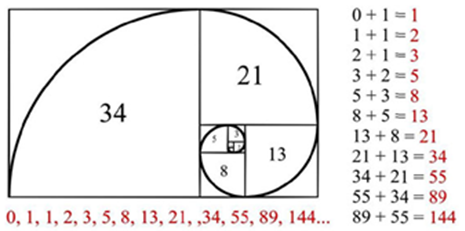
\includegraphics[width=0.45\textwidth]{c7_mutation_fs_01.png}\quad
    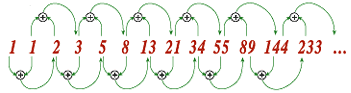
\includegraphics[width=0.4\textwidth]{c7_mutation_fs_02.png}
  \end{figure}
\end{frame}

\begin{frame}
  \frametitle{突变和随机化 | 生成随机DNA | 设计理念}
  \begin{figure}
    \centering
    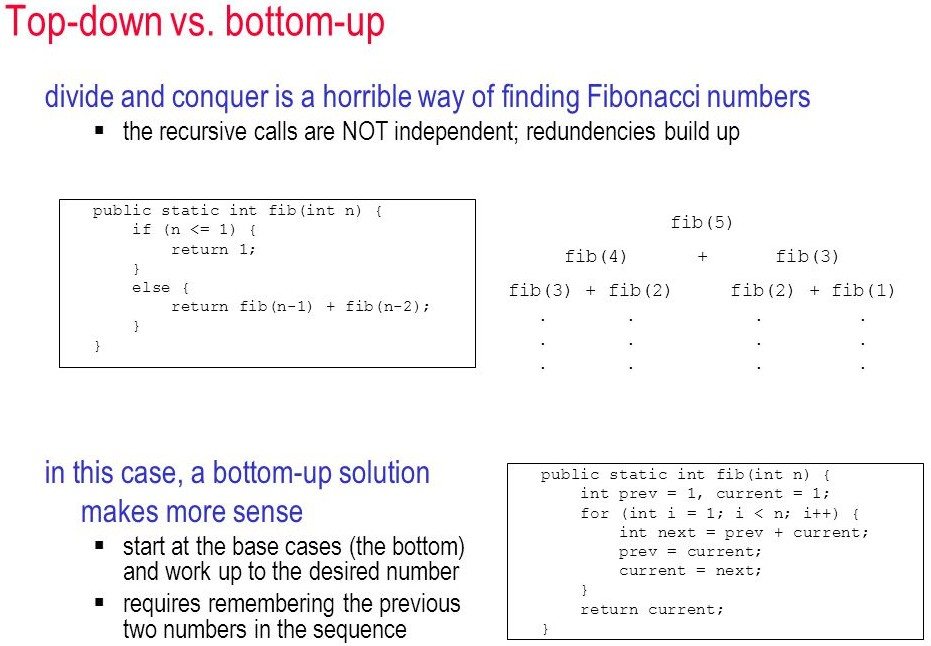
\includegraphics[width=0.9\textwidth]{c7_mutation_bt_01.jpg}
  \end{figure}
\end{frame}

\begin{frame}
  \frametitle{突变和随机化 | 生成随机DNA | 设计理念}
  \begin{figure}
    \centering
    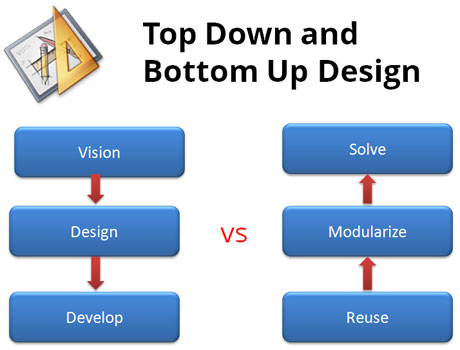
\includegraphics[width=0.53\textwidth]{c7_mutation_bt_02.jpg}
    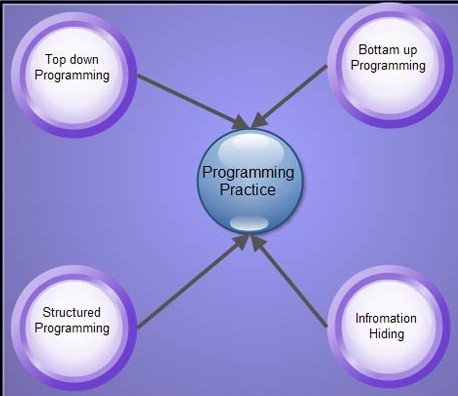
\includegraphics[width=0.43\textwidth]{c7_mutation_bt_03.jpg}
  \end{figure}
\end{frame}

\begin{frame}
  \frametitle{突变和随机化 | 生成随机DNA | 设计理念}
  \begin{figure}
    \centering
    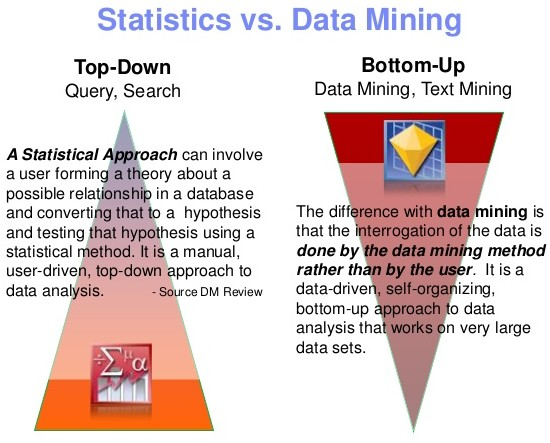
\includegraphics[width=0.38\textwidth]{c7_mutation_bt_04.jpg}
    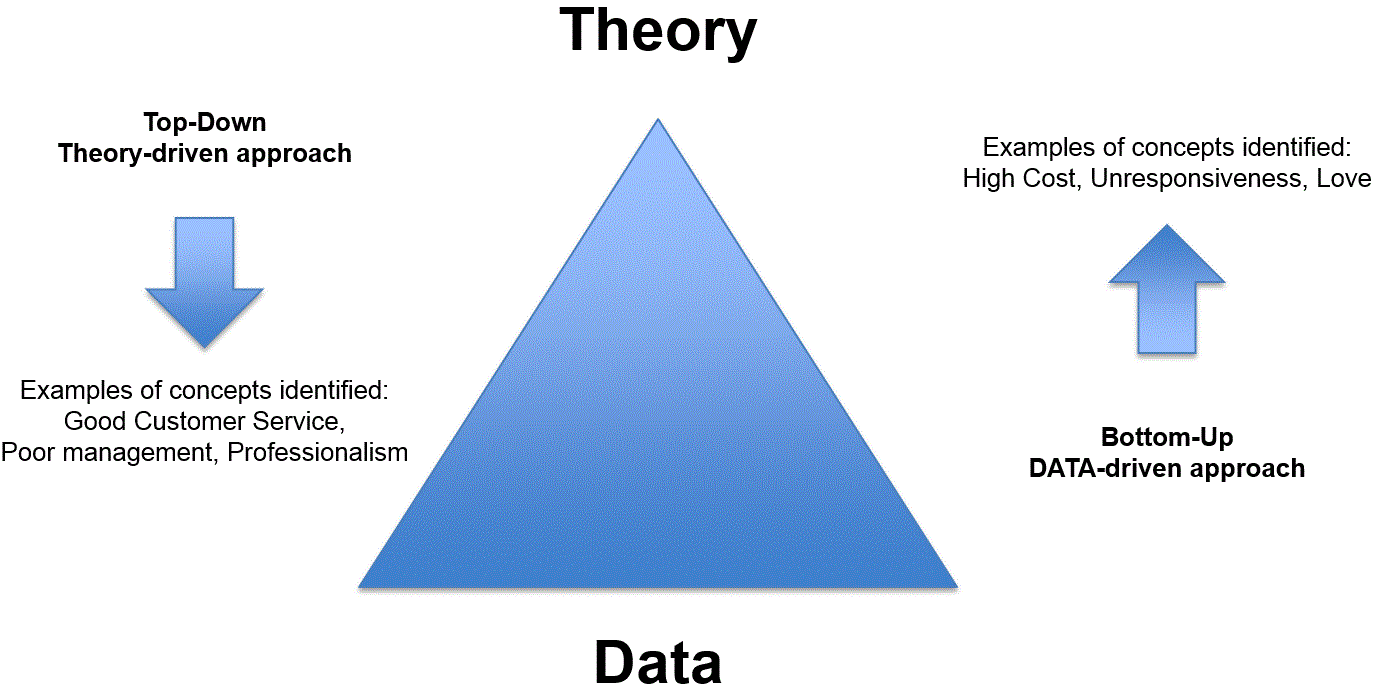
\includegraphics[width=0.58\textwidth]{c7_mutation_bt_05.png}
  \end{figure}
\end{frame}

\subsection{伪代码}
\begin{frame}[fragile]
  \frametitle{突变和随机化 | 生成随机DNA | 伪代码 | 自上而下S1}
  \begin{block}{目标}
    生成长短不一的随机DNA
  \end{block}
  \pause
  \begin{block}{途径}
  使用子程序 \verb|make_random_DNA_set| 直接生成数据
  \end{block}
  \pause
\begin{lstlisting}[language=]
@random_DNA = make_random_DNA_set( $minimum_length, $maximum_length, $size_of_set );
\end{lstlisting}
\end{frame}

\begin{frame}[fragile]
  \frametitle{突变和随机化 | 生成随机DNA | 伪代码 | 自上而下S2}
  \begin{block}{目标}
    编写 \verb|make_random_DNA_set| 子程序
  \end{block}
  \pause
\begin{lstlisting}[language=]
repeat $size_of_set times:

  $length = random number between minimum and maximum length

  $dna = make_random_DNA ( $length );

  add $dna to @set
}

return @set
\end{lstlisting}
\end{frame}

\begin{frame}[fragile]
  \frametitle{突变和随机化 | 生成随机DNA | 伪代码 | 自上而下S3}
  \begin{block}{目标}
    编写 \verb|make_random_DNA| 子程序
  \end{block}
  \pause
\begin{lstlisting}[language=]
from 1 to $length

  $base = randomnucleotide

  $dna .= $base
}

return $dna
\end{lstlisting}
\pause
\vspace{-0.5em}
  \begin{block}{目标}
    已经编写完了 \verb|randomnucleotide| 子程序
  \end{block}
\end{frame}

\subsection{程序}
\begin{frame}[fragile]
  \frametitle{突变和随机化 | 生成随机DNA | 程序7.3.1}
\begin{lstlisting}[firstnumber=1]
#!/usr/bin/perl -w
# Example 7-3   Generate random DNA
#  using a random number generator to randomly select bases

use strict;
use warnings;

# Declare and initialize the variables
my $size_of_set    = 12;
my $maximum_length = 30;
my $minimum_length = 15;
\end{lstlisting}
\end{frame}

\begin{frame}[fragile]
  \frametitle{突变和随机化 | 生成随机DNA | 程序7.3.2}
\begin{lstlisting}[firstnumber=13]
# An array, initialized to the empty list, to store the DNA in
my @random_DNA = ();

# Seed the random number generator.
# time|$$ combines the current time with the current process id
srand( time | $$ );

# And here's the subroutine call to do the real work
@random_DNA =
  make_random_DNA_set( $minimum_length, $maximum_length, $size_of_set );
\end{lstlisting}
\end{frame}

\begin{frame}[fragile]
  \frametitle{突变和随机化 | 生成随机DNA | 程序7.3.3}
\begin{lstlisting}[firstnumber=24]
# Print the results, one per line
print "Here is an array of $size_of_set randomly generated DNA sequences\n";
print "  with lengths between $minimum_length and $maximum_length:\n\n";

foreach my $dna (@random_DNA) {

    print "$dna\n";
}

print "\n";

exit;
\end{lstlisting}
\end{frame}

\begin{frame}[fragile]
  \frametitle{突变和随机化 | 生成随机DNA | 程序7.3.4}
\begin{lstlisting}[firstnumber=51]
sub make_random_DNA_set {

    # Collect arguments, declare variables
    my ( $minimum_length, $maximum_length, $size_of_set ) = @_;

    # length of each DNA fragment
    my $length;

    # DNA fragment
    my $dna;

    # set of DNA fragments
    my @set;
\end{lstlisting}
\end{frame}

\begin{frame}[fragile]
  \frametitle{突变和随机化 | 生成随机DNA | 程序7.3.5}
\begin{lstlisting}[firstnumber=65,basicstyle=\small\tt]
    # Create set of random DNA
    for ( my $i = 0 ; $i < $size_of_set ; ++$i ) {

        # find a random length between min and max
        $length = randomlength( $minimum_length, $maximum_length );

        # make a random DNA fragment
        $dna = make_random_DNA($length);

        # add $dna fragment to @set
        push( @set, $dna );
    }

    return @set;
}
\end{lstlisting}
\end{frame}

\begin{frame}[fragile]
  \frametitle{突变和随机化 | 生成随机DNA | 程序7.3.6}
\begin{lstlisting}[firstnumber=94,basicstyle=\small\tt]
sub randomlength {

    # Collect arguments, declare variables
    my ( $minlength, $maxlength ) = @_;

    # Calculate and return a random number within the
    #  desired interval.
    # Notice how we need to add one to make the endpoints inclusive,
    #  and how we first subtract, then add back, $minlength to
    #  get the random number in the correct interval.
    return ( int( rand( $maxlength - $minlength + 1 ) ) + $minlength );
}
\end{lstlisting}
\end{frame}

\begin{frame}[fragile]
  \frametitle{突变和随机化 | 生成随机DNA | 程序7.3.7}
\begin{lstlisting}[firstnumber=114]
sub make_random_DNA {

    # Collect arguments, declare variables
    my ($length) = @_;

    my $dna;

    for ( my $i = 0 ; $i < $length ; ++$i ) {

        $dna .= randomnucleotide();
    }

    return $dna;
}
\end{lstlisting}
\end{frame}

\begin{frame}[fragile]
  \frametitle{突变和随机化 | 生成随机DNA | 程序7.3.8}
\begin{lstlisting}[firstnumber=140]
sub randomnucleotide {

    my (@nucleotides) = ( 'A', 'C', 'G', 'T' );

    # scalar returns the size of an array.
    # The elements of the array are numbered 0 to size-1
    return randomelement(@nucleotides);
}
\end{lstlisting}
\end{frame}


\begin{frame}[fragile]
  \frametitle{突变和随机化 | 生成随机DNA | 程序7.3.9}
\begin{lstlisting}[firstnumber=156]
sub randomelement {

    my (@array) = @_;

    return $array[ rand @array ];
}
\end{lstlisting}
\end{frame}


\begin{frame}[fragile]
  \frametitle{突变和随机化 | 生成随机DNA | 程序7.3 | 输出}
\begin{lstlisting}[language=,basicstyle=\small\tt]
Here is an array of 12 randomly generated DNA sequences
  with lengths between 15 and 30:

TACGCTTGTGTTTTCGGGGGAC
GGGGTGTGGTAAGGCTGTCTCAGATGTGC
TGAACGACAACCTCCTGGACTTTACT
ATCTATGCTTTGCCATGCTAGT
CCGCTCATTCCTCTTCCTCGGC
TGTACCCCTAATACACTTTAGCCGAATTTA
ATAGGTCGGGGCGACAGCGCCGG
GATTGACCTCTGTAA
AAAATCTCTAGGATCGAGC
GTATGTGCTTGGGTAAAT
ATGGAGTTGCGAGGAAGTAGCTGAGT
GGCCCATGACCAGCATCCAGACAGCA
\end{lstlisting}
\end{frame}

\section{分析DNA}
\begin{frame}
  \frametitle{突变和随机化 | 分析DNA | 问题}
  \begin{figure}
    \centering
    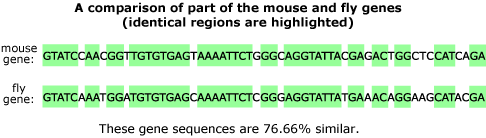
\includegraphics[width=0.9\textwidth]{c7_mutation_similar.png}
  \end{figure}
  \vspace{-1em}
  \begin{block}{一般性问题}
    两条DNA的相似性如何?(对于两个随机的DNA序列,平均来说,它们的碱基相同的百分比是多少?)
  \end{block}
  \pause
  \begin{block}{具体问题}
    \begin{itemize}
      \item 对于两条等长的DNA序列,同一位置碱基相同的百分比是多少?
      \item 对于一个DNA序列集来说,上述百分比的平均值是多少?
    \end{itemize}
  \end{block}
\end{frame}

\begin{frame}[fragile]
  \frametitle{突变和随机化 | 分析DNA | 伪代码}
\begin{lstlisting}[language=]
Generate a set of random DNA sequences, all the same length

For each pair of DNA sequences

  How many positions in the two sequences are identical as a fraction?

}

Report the mean of the preceding calculations as a percentage
\end{lstlisting}
\end{frame}

\begin{frame}[fragile]
  \frametitle{突变和随机化 | 分析DNA | 伪代码 | 比较相同位置上的核苷酸}
\begin{lstlisting}[language=]
assuming DNA1 is the same length as DNA2,

for each position from 1 to length(DNA)

  if the character at that position is the same in DNA_1 and DNA_2

    ++$count
  }
}

return count/length
\end{lstlisting}
\end{frame}

\begin{frame}[fragile]
  \frametitle{突变和随机化 | 分析DNA | 程序7.4.1}
\begin{lstlisting}[firstnumber=1]
#!/usr/bin/perl -w
# Example 7-4   Calculate the average percentage of positions that are the same
# between two random DNA sequences, in a set of 10 sequences.

use strict;
use warnings;

# Declare and initialize the variables
my $percent;
my @percentages;
my $result;
\end{lstlisting}
\end{frame}

\begin{frame}[fragile]
  \frametitle{突变和随机化 | 分析DNA | 程序7.4.2}
\begin{lstlisting}[firstnumber=13]
# An array, initialized to the empty list, to store the DNA in
my @random_DNA = ();

# Seed the random number generator.
# time|$$ combines the current time with the current process id
srand( time | $$ );

#  Generate the data set of 10 DNA sequences.
@random_DNA = make_random_DNA_set( 10, 10, 10 );
\end{lstlisting}
\end{frame}

\begin{frame}[fragile]
  \frametitle{突变和随机化 | 分析DNA | 程序7.4.3}
\begin{lstlisting}[firstnumber=23]
# Iterate through all pairs of sequences
for ( my $k = 0 ; $k < scalar @random_DNA - 1 ; ++$k ) {
    for ( my $i = ( $k + 1 ) ; $i < scalar @random_DNA ; ++$i ) {

        # Calculate and save the matching percentage
        $percent = matching_percentage( $random_DNA[$k], $random_DNA[$i] );
        push( @percentages, $percent );
    }
}
\end{lstlisting}
\end{frame}

\begin{frame}[fragile]
  \frametitle{突变和随机化 | 分析DNA | 程序7.4.4}
  \vspace{-0.5em}
\begin{lstlisting}[firstnumber=33]
# Finally, the average result:
$result = 0;

foreach $percent (@percentages) {
    $result += $percent;
}

$result = $result / scalar(@percentages);

#Turn result into a true percentage
$result = int( $result * 100 );
print "In this run of the experiment, the average percentage of \n";
print "matching positions is $result%\n\n";

exit;
\end{lstlisting}
\end{frame}

\begin{frame}[fragile]
  \frametitle{突变和随机化 | 分析DNA | 程序7.4.5}
\begin{lstlisting}[firstnumber=58]
sub matching_percentage {

    my ( $string1, $string2 ) = @_;

    # we assume that the strings have the same length
    my ($length) = length($string1);
    my ($position);
    my ($count) = 0;
\end{lstlisting}
\end{frame}

\begin{frame}[fragile]
  \frametitle{突变和随机化 | 分析DNA | 程序7.4.6}
\begin{lstlisting}[firstnumber=67]
    for ( $position = 0 ; $position < $length ; ++$position ) {
        if (
            substr( $string1, $position, 1 ) eq substr( $string2, $position, 1 )
          )
        {
            ++$count;
        }
    }

    return $count / $length;
}
\end{lstlisting}
\end{frame}

\begin{frame}[fragile]
  \frametitle{突变和随机化 | 分析DNA | 程序7.4.7}
\begin{lstlisting}[firstnumber=89]
sub make_random_DNA_set {

    # Collect arguments, declare variables
    my ( $minimum_length, $maximum_length, $size_of_set ) = @_;

    # length of each DNA fragment
    my $length;

    # DNA fragment
    my $dna;

    # set of DNA fragments
    my @set;
\end{lstlisting}
\end{frame}

\begin{frame}[fragile]
  \frametitle{突变和随机化 | 分析DNA | 程序7.4.8}
\begin{lstlisting}[firstnumber=103,basicstyle=\small\tt]
    # Create set of random DNA
    for ( my $i = 0 ; $i < $size_of_set ; ++$i ) {

        # find a random length between min and max
        $length = randomlength( $minimum_length, $maximum_length );

        # make a random DNA fragment
        $dna = make_random_DNA($length);

        # add $dna fragment to @set
        push( @set, $dna );
    }

    return @set;
}
\end{lstlisting}
\end{frame}

\begin{frame}[fragile]
  \frametitle{突变和随机化 | 分析DNA | 程序7.4.9}
\begin{lstlisting}[firstnumber=127,basicstyle=\small\tt]
sub randomlength {

    # Collect arguments, declare variables
    my ( $minlength, $maxlength ) = @_;

    # Calculate and return a random number within the
    #  desired interval.
    # Notice how we need to add one to make the endpoints inclusive,
    #  and how we first subtract, then add back, $minlength to
    #  get the random number in the correct interval.
    return ( int( rand( $maxlength - $minlength + 1 ) ) + $minlength );
}
\end{lstlisting}
\end{frame}

\begin{frame}[fragile]
  \frametitle{突变和随机化 | 分析DNA | 程序7.4.10}
\begin{lstlisting}[firstnumber=147]
sub make_random_DNA {

    # Collect arguments, declare variables
    my ($length) = @_;

    my $dna;

    for ( my $i = 0 ; $i < $length ; ++$i ) {
        $dna .= randomnucleotide();
    }

    return $dna;
}
\end{lstlisting}
\end{frame}

\begin{frame}[fragile]
  \frametitle{突变和随机化 | 分析DNA | 程序7.4.11}
\begin{lstlisting}[firstnumber=168]
sub randomnucleotide {

    my (@nucleotides) = ( 'A', 'C', 'G', 'T' );

    # scalar returns the size of an array.
    # The elements of the array are numbered 0 to size-1
    return randomelement(@nucleotides);
}
\end{lstlisting}
\end{frame}

\begin{frame}[fragile]
  \frametitle{突变和随机化 | 分析DNA | 程序7.4.12}
\begin{lstlisting}[firstnumber=184]
sub randomelement {

    my (@array) = @_;

    return $array[ rand @array ];
}
\end{lstlisting}
\end{frame}

\begin{frame}[fragile]
  \frametitle{突变和随机化 | 分析DNA | 程序7.4 | \alert{子程序}}
  \vspace{-0.5em}
\begin{lstlisting}
sub matching_percentage {
    my ( $string1, $string2 ) = @_;
    my ($length) = length($string1);
    my ($position); my ($count) = 0;
    for ( $position = 0 ; $position < $length ; ++$position ) {
        if (
            substr( $string1, $position, 1 ) eq substr( $string2, $position, 1 )
          )
        {
            ++$count;
        }
    }
    return $count / $length;
}
\end{lstlisting}
\end{frame}

\begin{frame}[fragile]
  \frametitle{突变和随机化 | 分析DNA | 程序7.4 | 输出}
\begin{lstlisting}[firstnumber=1]
In this run of the experiment, the average number of 
matching positions is 24%
\end{lstlisting}
\end{frame}

\begin{frame}
  \frametitle{突变和随机化 | 分析DNA | 程序7.4 | 输出 | 25\%?}
  \begin{figure}
    \centering
    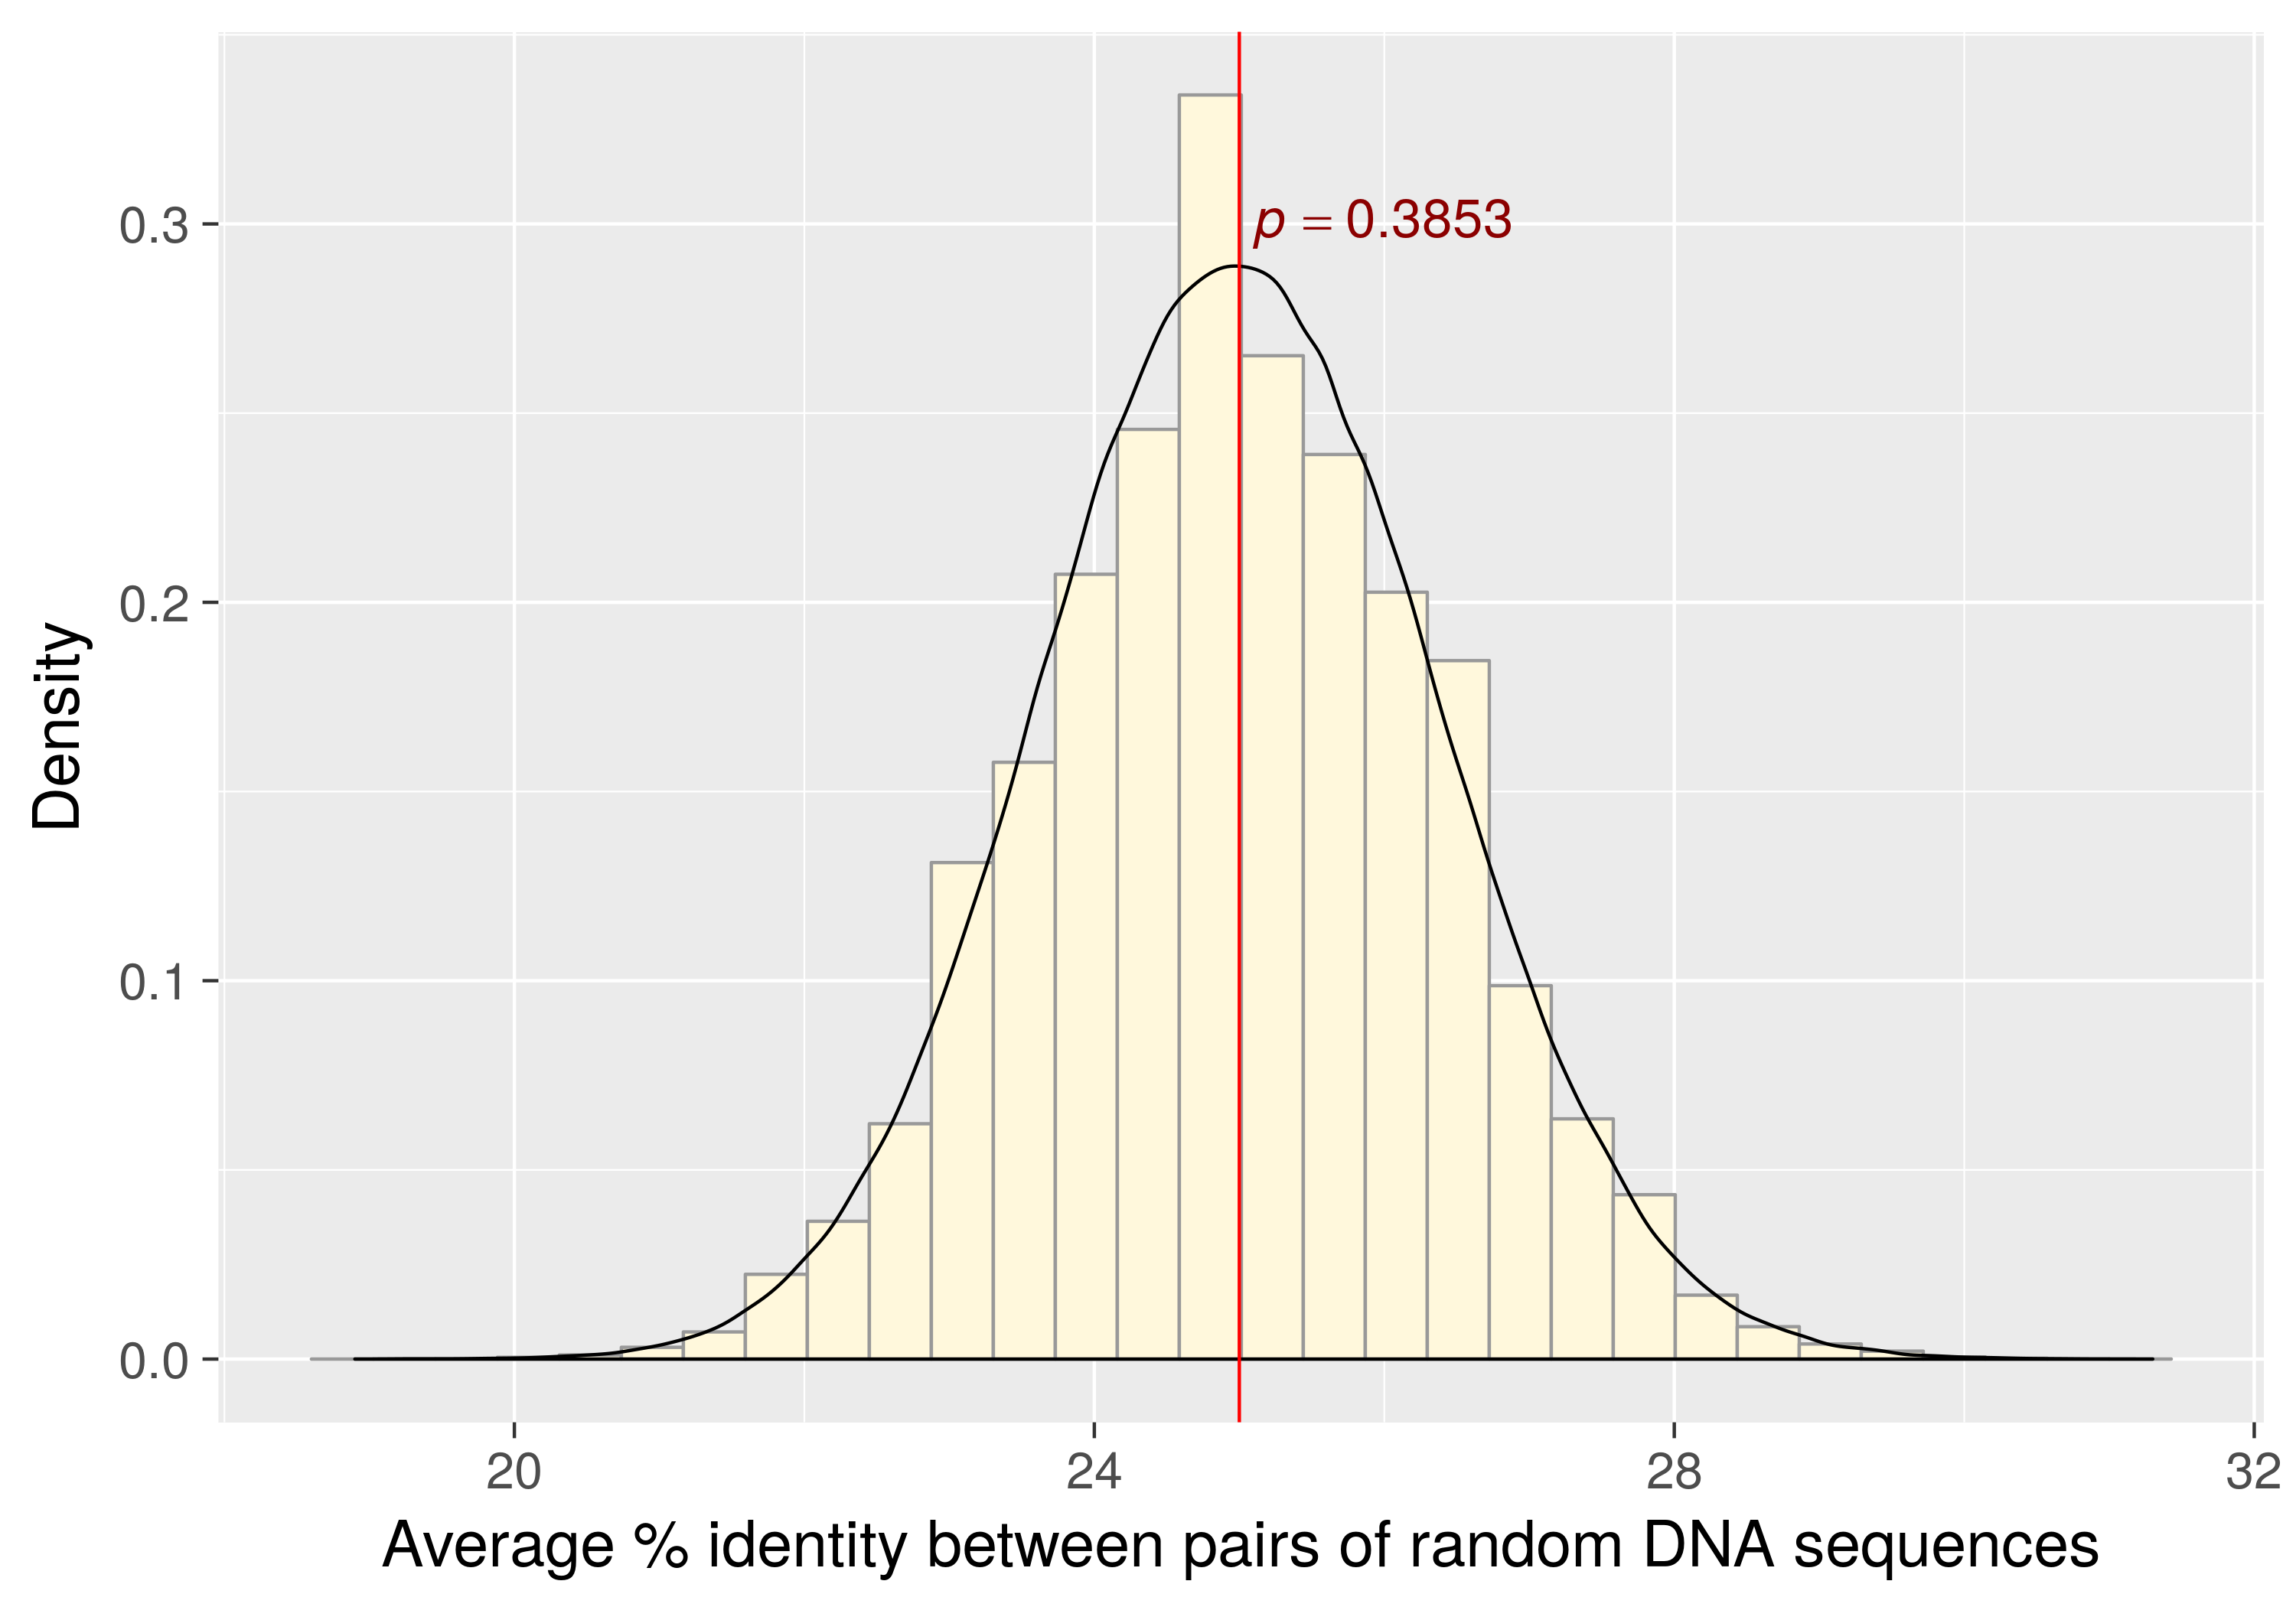
\includegraphics[width=0.9\textwidth]{c7_mutation_similar_plot.png}
  \end{figure}
\end{frame}

\begin{frame}[fragile]
  \frametitle{突变和随机化 | 分析DNA | 程序7.4 | 子程序调用}
\begin{lstlisting}
@random_DNA = make_random_DNA_set( 10, 10, 10 );
\end{lstlisting}
\pause
\begin{lstlisting}
my $minimum_length = 10;
my $maximum_length = 10;
my $size_of_set    = 10;

@random_DNA = make_random_DNA_set( $minimum_length, $maximum_length, $size_of_set );
\end{lstlisting}
\end{frame}

\begin{frame}[fragile]
  \frametitle{突变和随机化 | 分析DNA | 程序7.4 | \alert{嵌套循环}}
\begin{lstlisting}
# Iterate through all pairs of sequences
for (my $k = 0 ; $k < scalar @random_DNA - 1 ; ++$k) {
  for (my $i = ($k + 1) ; $i < scalar @random_DNA ; ++$i) {

    # Calculate and save the matching percentage
    $percent = matching_percentage($random_DNA[$k], $random_DNA[$i]);
    push(@percentages, $percent);
  }
}
\end{lstlisting}
\end{frame}

\begin{frame}
  \frametitle{突变和随机化 | 分析DNA | 程序7.4 | 嵌套循环}
  \begin{figure}
    \centering
    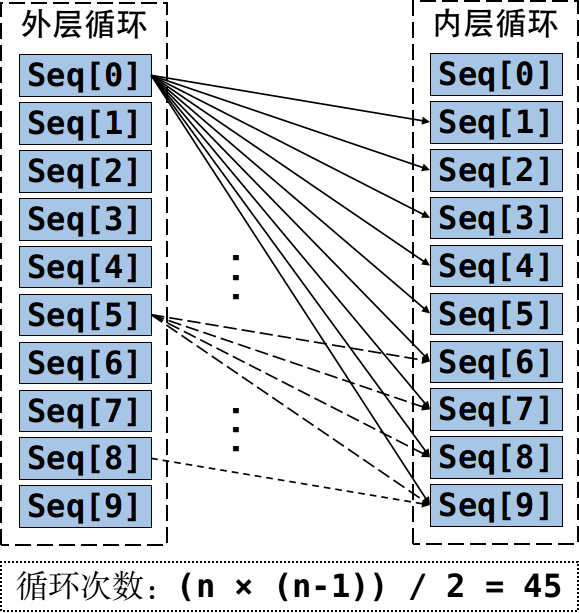
\includegraphics[width=0.7\textwidth,height=0.8\textheight]{c7_mutation_nested_loop.png}
  \end{figure}
\end{frame}

\begin{frame}
  \frametitle{突变和随机化 | 分析DNA | 程序7.4 | 嵌套循环}
  \begin{figure}
    \centering
    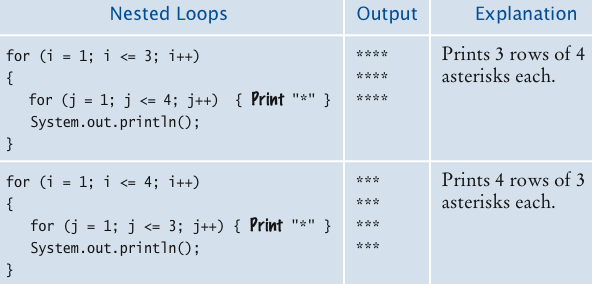
\includegraphics[width=0.9\textwidth]{c7_mutation_nl_01.png}
  \end{figure}
\end{frame}

\begin{frame}
  \frametitle{突变和随机化 | 分析DNA | 程序7.4 | 嵌套循环}
  \begin{figure}
    \centering
    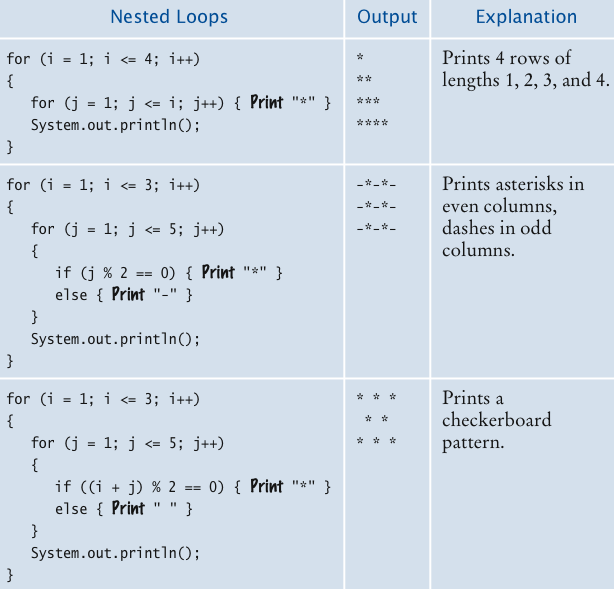
\includegraphics[width=0.68\textwidth]{c7_mutation_nl_02.png}
  \end{figure}
\end{frame}

\begin{frame}
  \frametitle{突变和随机化 | 分析DNA | 程序7.4 | 嵌套循环}
  \begin{figure}
    \centering
    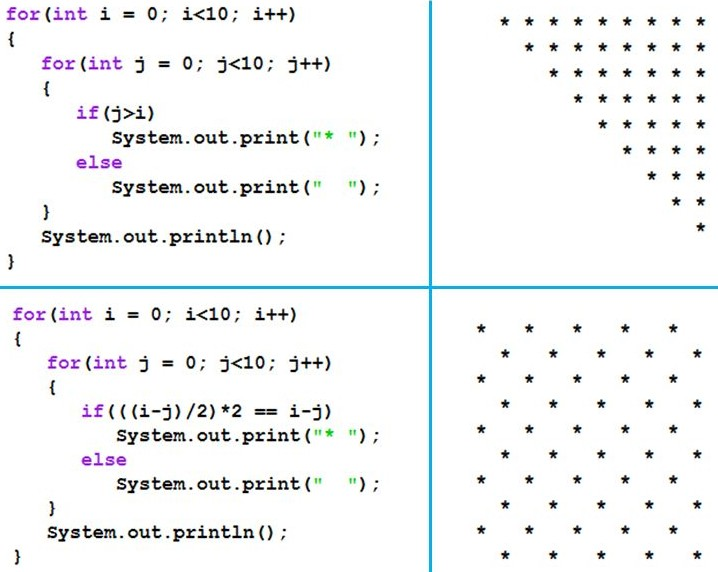
\includegraphics[width=0.8\textwidth]{c7_mutation_nl_03.jpg}
  \end{figure}
\end{frame}

\section{知识拓展}
\begin{frame}
  \frametitle{突变和随机化 | 知识拓展 | 嵌套}
  \begin{figure}
    \centering
    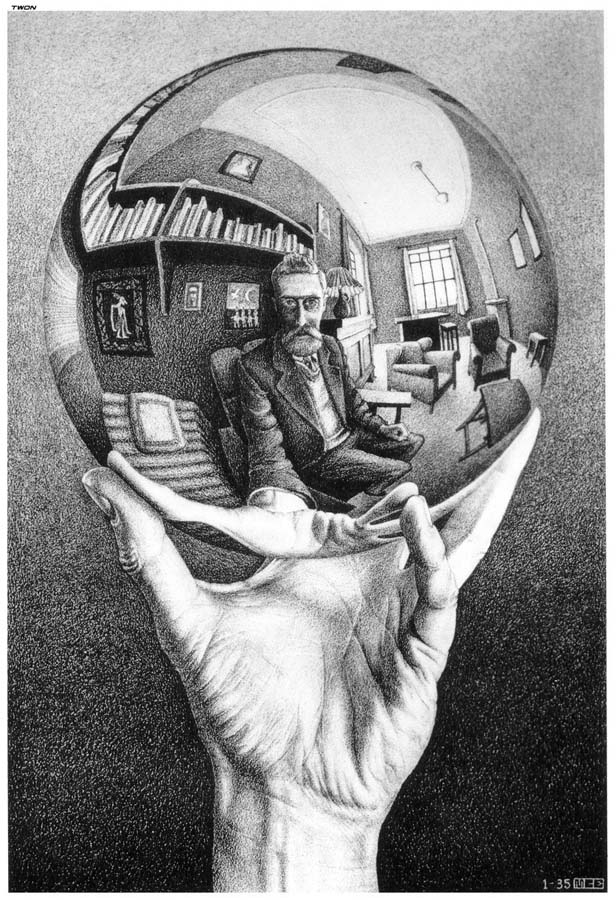
\includegraphics[width=0.39\textwidth]{c7_mutation_supp_01.jpg}\quad
    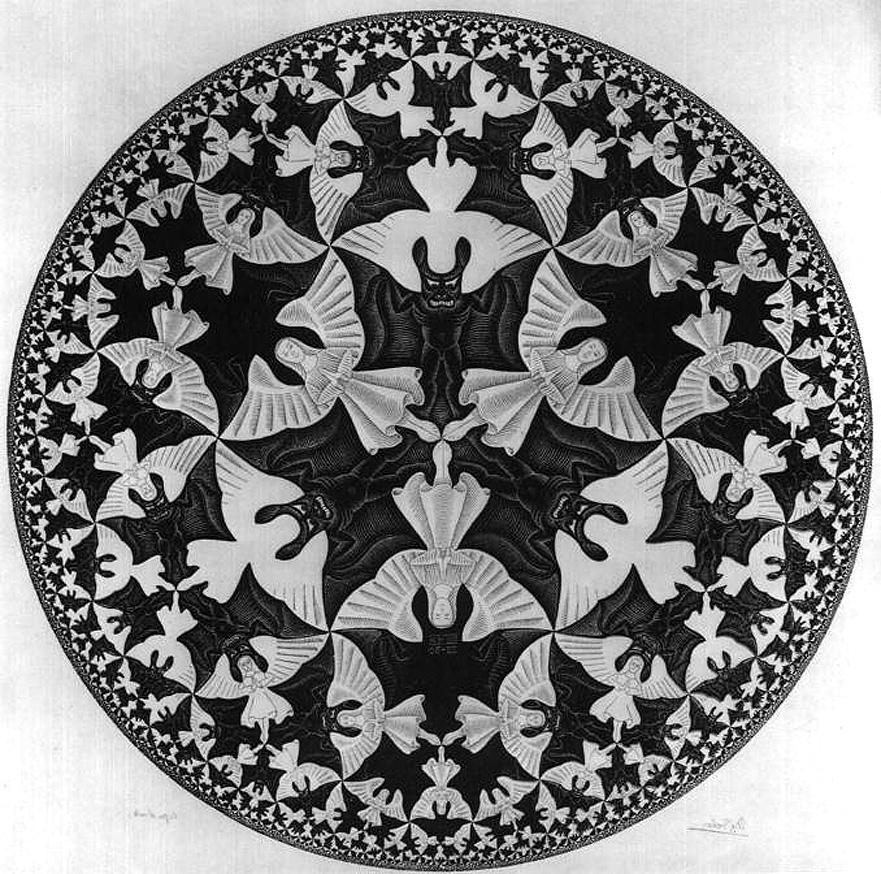
\includegraphics[width=0.56\textwidth]{c7_mutation_supp_02.jpg}
  \end{figure}
\end{frame}

\begin{frame}
  \frametitle{突变和随机化 | 知识拓展 | 死循环}
  \begin{figure}
    \centering
    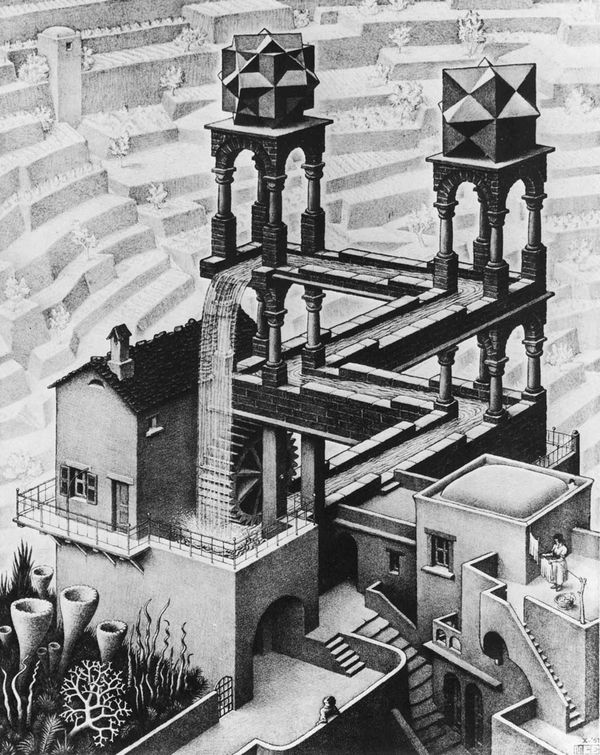
\includegraphics[width=0.34\textwidth]{c7_mutation_supp_05.jpg}\quad
    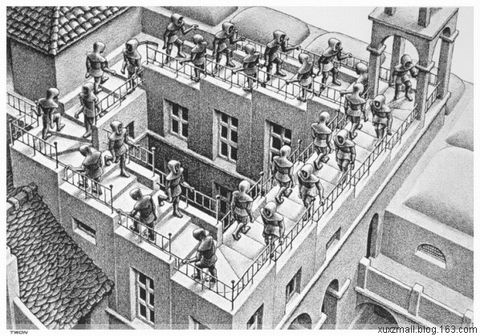
\includegraphics[width=0.62\textwidth]{c7_mutation_supp_06.jpg}
  \end{figure}
\end{frame}

\begin{frame}
  \frametitle{突变和随机化 | 知识拓展 | 死循环}
  \begin{figure}
    \centering
    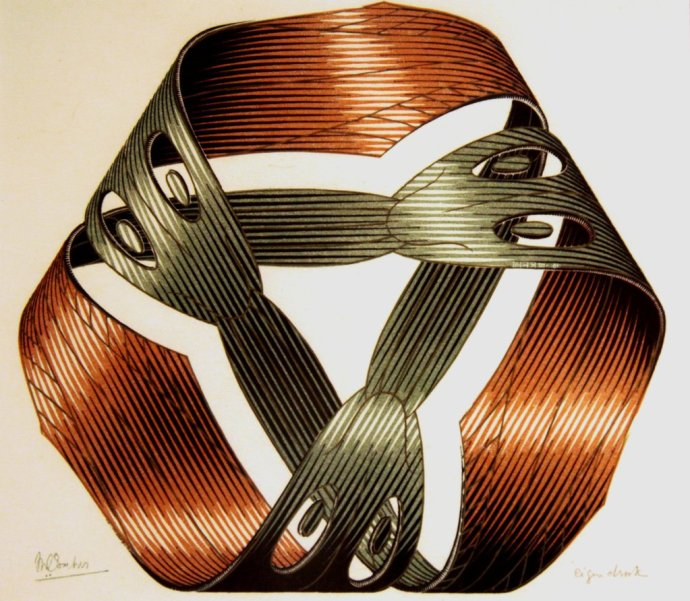
\includegraphics[width=0.39\textwidth]{c7_mutation_supp_20.jpg}\quad
    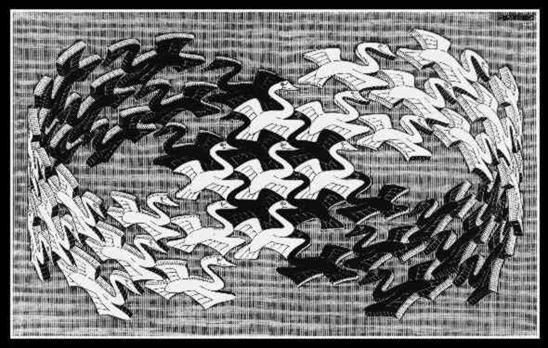
\includegraphics[width=0.53\textwidth]{c7_mutation_supp_21.jpg}
  \end{figure}
\end{frame}

\begin{frame}
  \frametitle{突变和随机化 | 知识拓展 | 死循环}
  \begin{columns}
    \column{0.3\textwidth}
    \begin{block}{莫比乌斯带}
      \begin{figure}
        \centering
        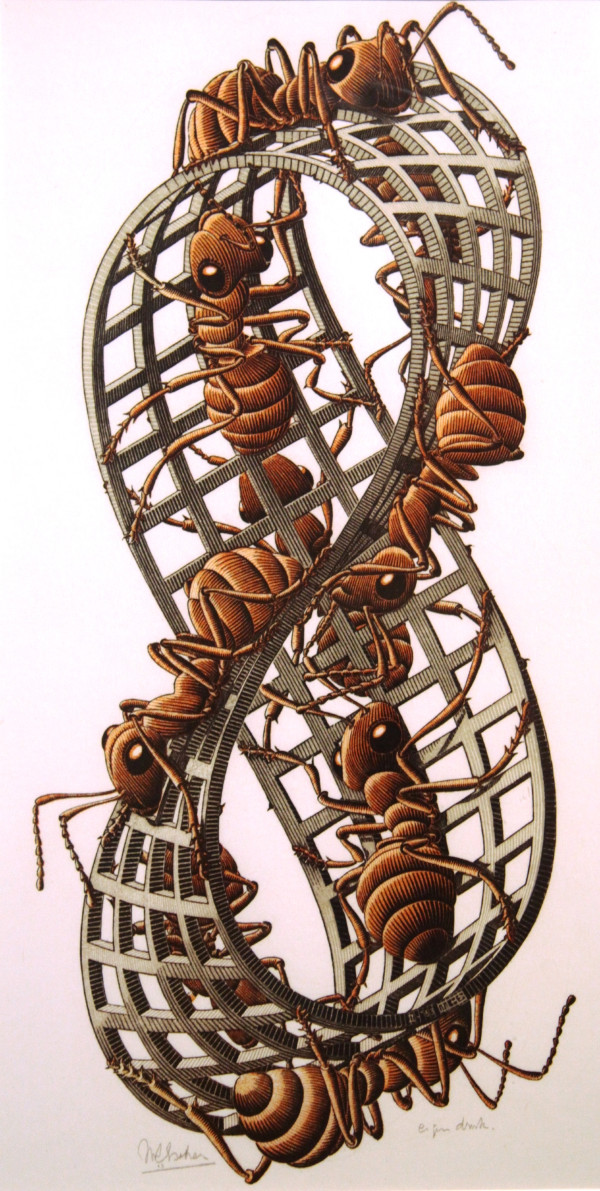
\includegraphics[width=0.9\textwidth]{c7_mutation_supp_22.jpg}
      \end{figure}
    \end{block}
    \column{0.3\textwidth}
    \begin{block}{克莱因瓶}
      \begin{figure}
        \centering
        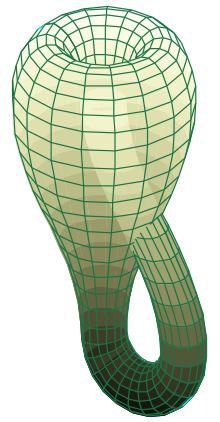
\includegraphics[width=0.93\textwidth]{c7_mutation_supp_23.png}
      \end{figure}
    \end{block}
    \column{0.3\textwidth}
    \begin{block}{潘洛斯三角}
      \begin{figure}
        \centering
        
\includegraphics[width=0.9\textwidth]{c7_mutation_supp_24.png}
      \end{figure}
    \end{block}
  \end{columns}
\end{frame}

\begin{frame}
  \frametitle{突变和随机化 | 知识拓展 | 递归}
  \begin{figure}
    \centering
    
\includegraphics[width=0.49\textwidth]{c7_mutation_supp_07.jpg}\quad
    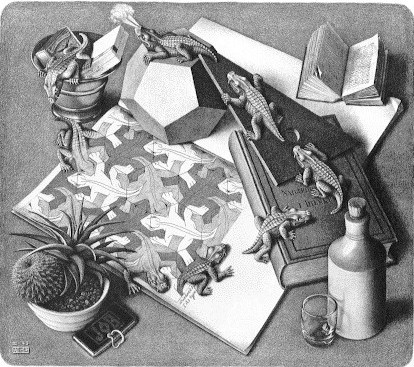
\includegraphics[width=0.47\textwidth]{c7_mutation_supp_08.jpg}
  \end{figure}
\end{frame}

\begin{frame}
  \frametitle{突变和随机化 | 知识拓展 | GEB}
  \begin{figure}
    \centering
    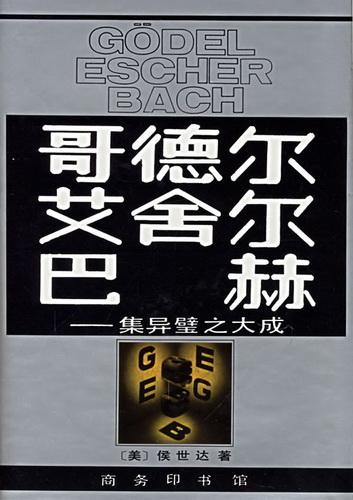
\includegraphics[width=0.45\textwidth]{c7_mutation_supp_09.jpg}
  \end{figure}
\end{frame}

\begin{frame}
  \frametitle{突变和随机化 | 知识拓展 | GEB}
  \begin{block}{《哥德尔、埃舍尔、巴赫》}
    《哥德尔、埃舍尔、巴赫:集异璧之大成》(Gödel, Escher, Bach: an Eternal Golden Braid),是一本赢得普立兹奖的书。它是侯世达的著作,由Basic Books出版社在1979年出版的。这本书的二十周年版本在1999年发行,而且由侯世达加上新的前言。《集异璧之大成》(ISBN 7-100-01323-2)是商务印书馆在1996年出版的根据1995年英文版翻译的中文版。\\
    \vspace{0.3em}
本书的英文副标题意译为“一条永恒的金带”,其首字母与哥德尔、埃舍尔、巴赫三人的英文名字首字母GEB相同,而商务印书馆中文译本的副标题中的“集异璧”则与GEB谐音。本书一共有两篇,上篇译为“集异璧GEB”,下篇译为“异集璧EGB”。 \\
    \vspace{0.3em}
本书主要讲述了逻辑学家哥德尔、艺术家埃舍尔和作曲家巴赫的创造性的成就怎样交织在一起。正如作者所说:“我认识到,哥德尔、埃舍尔和巴赫只是用不同的方式来表达一样相同的本质。我尝试重现这种本质而写出这本书。”
  \end{block}
\end{frame}

\begin{frame}
  \frametitle{突变和随机化 | 知识拓展 | GEB | 侯世达}
  \begin{block}{侯世达}
    侯世达因其著作《哥德尔、埃舍尔、巴赫》获得普立兹奖(非小说类别)和美国国家图书奖(科学类别)。
  \end{block}
  \begin{block}{\alert{侯世达定律}}
    侯世达定律(Hofstadter's law)是一句自指的格言,由侯世达在《哥德尔、埃舍尔、巴赫》一书中提出:
    \begin{quote}
    侯世达定律:做事所花费的时间总是比你预期的要长,即使你的预期中考虑了侯世达定律。 ——侯世达,《哥德尔、埃舍尔、巴赫》
    \end{quote}
\\侯世达定律指做复杂任务需要花费的时间总是很难预计的。程序员经常会引用这一定律,特别是在进行有关提高效率的讨论时(如《人月神话》和极限编程)。其自指的特征反映了即便意识到任务的复杂性,预计花费的时间仍是困难的。
  \end{block}
\end{frame}

\begin{frame}[fragile]
  \frametitle{图标和随机化 | 知识拓展 | 斐波那契数列 | 递归}
\begin{lstlisting}
#!/usr/bin/perl

use strict;
use warnings;

sub F {
    my $n = shift;
    return 0 if $n == 0;
    return 1 if $n == 1;
    return F( $n - 1 ) + F( $n - 2 );
}

print F( $ARGV[0] ), "\n";
\end{lstlisting}
\end{frame}

\begin{frame}[fragile]
  \frametitle{图标和随机化 | 知识拓展 | 斐波那契数列 | \alert{闭包 $\Rightarrow$ 缓存}}
  \vspace{-0.5em}
\begin{lstlisting}[basicstyle=\small\tt]
#!/usr/bin/perl

use strict; use warnings;

{
    my %fib;
    sub F {
        my $n = shift;
        return 0 if $n == 0;
        return 1 if $n == 1;
        if ( not exists $fib{$n} ) {
            $fib{$n} = F( $n - 1 ) + F( $n - 2 );
        }
        return $fib{$n};
    }
}

print F( $ARGV[0] ), "\n";
\end{lstlisting}
\end{frame}

\begin{frame}[fragile]
  \frametitle{图标和随机化 | 知识拓展 | 斐波那契数列 | 模块 $\Rightarrow$ 缓存}
\begin{lstlisting}
#!/usr/bin/perl

use strict; use warnings;
use Memoize;

memoize('F');

sub F {
    my $n = shift;
    return 0 if $n == 0;
    return 1 if $n == 1;
    return F( $n - 1 ) + F( $n - 2 );
}

print F( $ARGV[0] ), "\n";
\end{lstlisting}
\end{frame}

\begin{frame}[fragile]
  \frametitle{图标和随机化 | 知识拓展 | 斐波那契数列 | 总结}
  \vspace{-0.5em}
  \begin{lstlisting}[basicstyle=\small\tt]
# 1. Compute Fibonacci numbers
sub fib {
  my $n = shift;
  return $n if $n < 2;
  fib($n-1) + fib($n-2);
}
# 2. Compute Fibonacci numbers, memoized version
{ my @fib;
  sub fib {
    my $n = shift;
    return $fib[$n] if defined $fib[$n];
    return $fib[$n] = $n if $n < 2;
    $fib[$n] = fib($n-1) + fib($n-2);
  }
}
# 3. Compute Fibonacci numbers, module version
use Memoize;
memoize('fib');
\end{lstlisting}
\end{frame}

\section{回顾和总结}
\subsection{总结}
\begin{frame}
  \frametitle{突变和随机化 | 总结}
  \begin{block}{知识点}
    \begin{itemize}
      \item 随机:数组的随机元素,字符串的随机位置,两个整数间的随机数
      \item 随机数生成器:伪随机,种子
      \item 程序设计理念:自上而下,自下而上
      \item 其他:do-until,变量声明,嵌套循环
    \end{itemize}
  \end{block}
  \pause
  \begin{block}{技能}
    \begin{itemize}
      \item 熟练使用Perl语言中的随机数生成器
      \item 熟练分割任务、设计子程序
      \item 熟练使用自下而上和自上而下的理念设计程序
      \item 能够用Perl语言编写DNA突变相关的程序
    \end{itemize}
  \end{block}
\end{frame}

\subsection{思考题}
\begin{frame}
  \frametitle{突变和随机化 | 思考题}
  \begin{enumerate}
    \item 在Perl语言中如何设置随机数生成器的种子?
    \item 如何随机选取数组的元素?
    \item 如何随机选取字符串的位置?
    \item 如何随机选取两个整数间的一个数字?
    \item 比较自下而上和自上而下两种设计理念。
    \item 解释嵌套循环的工作步骤。
  \end{enumerate}
\end{frame}

\begin{frame}
  \frametitle{下节预告}
  \begin{block}{计算机}
    回顾总结常见的排序和查找算法。
  \end{block}
  \begin{block}{生物}
    回顾遗传密码、翻译和阅读框的相关知识。
  \end{block}
\end{frame}


\input{snippet/class_tail.tex}
